\documentclass[a4paper,12pt]{report}
\usepackage[utf8]{vietnam}
\usepackage{geometry}
\usepackage{amsmath}
\usepackage{enumitem}
\usepackage{booktabs}
\usepackage{array}
\usepackage{parskip}
\usepackage{hyperref}
\usepackage{graphicx}
\usepackage{tocbibind} % Để thêm mục lục, tài liệu tham khảo vào mục lục
\usepackage{float} % Thêm gói float để sử dụng [H]

% Thiết lập lề trang
\geometry{a4paper, left=3cm, right=2cm, top=2.5cm, bottom=2.5cm}

% Tắt thụt đầu dòng
\setlength{\parindent}{0pt}

% Thiết lập khoảng cách dòng
\linespread{1.2}

\begin{document}

% Trang bìa
\begin{titlepage}
    \centering

    \huge
    \textbf{TRƯỜNG ĐẠI HỌC SÀI GÒN} \\[0.3cm]
    \large
    \textbf{KHOA CÔNG NGHỆ THÔNG TIN} \\[1cm]
    
    
\includegraphics[width=9cm]{SGU-LOGO.png} \\[1cm]
    \Large
    \textbf{BÁO CÁO ĐỒ ÁN CUỐI KỲ} \\[0.3cm]
    \Large
    \textbf{Học Phần: Trí Tuệ Nhân Tạo Nâng Cao (841458)} \\[0.5cm]
    
    \textbf{Chủ Đề: Xây dựng và đánh giá Game AI đa cấp độ - Extended Tic-Tac-Toe} \\[0.7cm]
    
    \textbf{Sinh Viên Thực Hiện:} \\[0.3cm]
    \begin{tabular}{ll}
        Trương Chí Long & MSSV: 3123410198 \\
    \end{tabular} \\[0.5cm]
    \Large
    \text{Giảng Viên Hướng Dẫn:} \textbf{Đỗ Như Tài} \\[2cm]
    \normalsize
    \textbf{Thành phố Hồ Chí Minh, tháng 11 năm 2026}
    \vfill
\end{titlepage}

% Mục lục tự động
\tableofcontents
\clearpage
\renewcommand{\thesection}{\arabic{section}}

% ==============================================================================
% CHƯƠNG 1: GIỚI THIỆU & ĐẶT VẤN ĐỀ NGHIÊN CỨU
% ==============================================================================
\section{Giới thiệu \& Đặt vấn đề Nghiên cứu}

\subsection{Bối cảnh \& Động lực Nghiên cứu}
Trò chơi cờ ca-rô cổ điển Tic-Tac-Toe trên bàn cờ $3 \times 3$ với điều kiện thắng $K=3$ là bài toán nhập môn kinh điển trong lý thuyết trò chơi đối kháng và Trí tuệ nhân tạo. Tuy nhiên, xét dưới góc độ thực nghiệm thuật toán nâng cao, biến thể $3 \times 3$ truyền thống bộc lộ ba giới hạn nghiêm trọng:
\begin{itemize}[leftmargin=1.2cm]
    \item \textbf{Không gian trạng thái cực nhỏ:} Toàn bộ bàn cờ chỉ có tối đa $3^9 = 19{,}683$ cấu hình trạng thái và không quá $9! = 362{,}880$ chuỗi nước đi hợp lệ (theo kết quả giải chuẩn còn $4{,}520$ trạng thái chính quy có thể tiếp cận).
    \item \textbf{Dễ dàng vét cạn và cân bằng tuyệt đối:} Các thuật toán tìm kiếm cổ điển như Minimax hoặc cắt tỉa Alpha-Beta dễ dàng duyệt trọn vẹn cây trò chơi đến trạng thái kết thúc. Khi cả hai tác tử đều chơi tối ưu, trò chơi hội tụ hoàn toàn về kết quả hòa, khiến năng lực chiến thuật không thể phân hóa sâu hơn.
    \item \textbf{Làm mờ ranh giới đánh giá các phương pháp học máy:} Trên không gian hẹp $3 \times 3$, một hệ luật Heuristic đơn giản hay một bảng tra cứu nhỏ đều có thể tiệm cận trạng thái bất bại, làm lu mờ sự khác biệt thực chất giữa Heuristic tĩnh, Học có giám sát (Supervised Learning), Học tăng cường (Reinforcement Learning) và Tìm kiếm cây Monte Carlo (MCTS).
\end{itemize}

Để tạo ra một môi trường thực nghiệm có giá trị khoa học và bộc lộ đầy đủ bản chất của từng lớp thuật toán, đồ án mở rộng bài toán lên không gian tổng quát \textbf{Extended Tic-Tac-Toe ($M \times N, K$)}, trong đó $M \times N$ là kích thước bàn cờ và $K$ là số quân liên tiếp cần thiết để chiến thắng theo một trong bốn trục (ngang, dọc, chéo chính, chéo phụ). Đồ án lựa chọn cấu hình \textbf{$4 \times 4, K=4$} làm chuẩn thực nghiệm chính (Primary Benchmark), đồng thời hỗ trợ đối chứng trên $4 \times 4, K=3$, $3 \times 3, K=3$ và mở rộng tổng quát hóa lên $5 \times 5, K=4$.

Trên bàn cờ $4 \times 4, K=4$, không gian trạng thái tăng vọt lên $3^{16} \approx 4.3 \times 10^7$ cấu hình và cây trò chơi có thể đạt tới $16! \approx 2.09 \times 10^{13}$ chuỗi nước đi. Sự bùng nổ tổ hợp nhánh tìm kiếm $O(b^d)$ khiến việc tìm kiếm vét cạn toàn cây trong thời gian thực trở nên bất khả thi, qua đó làm bộc lộ rõ nét:
\begin{enumerate}[leftmargin=1.2cm]
    \item Giá trị của hàm lượng giá Heuristic tĩnh và hiệu quả cắt giảm không gian tìm kiếm từ kỹ thuật cắt tỉa Alpha-Beta kết hợp sắp xếp nước đi (Move Ordering).
    \item Cơ chế lấy mẫu định hướng và đánh đổi giữa khám phá với khai thác trong Tìm kiếm cây Monte Carlo (MCTS UCT).
    \item Khả năng xấp xỉ hàm chính sách/giá trị của Mạng Nơ-ron tích chập (CNN) và Học tăng cường tự chơi (DQN Self-Play) trên không gian lớn hơn khả năng lưu bảng tường minh.
    \item Hiệu quả cộng hưởng của mô hình lai (Hybrid MCTS) kết hợp tri thức tiên nghiệm từ mạng học sâu với tìm kiếm cây đối kháng theo hướng cảm hứng từ AlphaGo.
\end{enumerate}

\subsection{Mục tiêu Kỹ thuật \& Đóng góp Cốt lõi của Đề tài}
Đề tài được thiết kế và hoàn thiện với bốn mục tiêu kỹ thuật cốt lõi:
\begin{itemize}[leftmargin=1.2cm]
    \item \textbf{Xây dựng Game Engine tổng quát $M \times N, K$ chuẩn mực:} Phân tách độc lập tầng lõi trò chơi khỏi các thư viện AI/UI, tuân thủ mô hình Markov Decision Process (MDP) với hợp đồng API chuẩn hóa và đạt 100\% bộ kiểm thử đơn vị tự động.
    \item \textbf{Hiện thực hóa hệ sinh thái 7 cấp độ tác tử AI:} Thiết kế, cài đặt đầy đủ và giải thích tường minh từ gốc 7 cấp độ tác tử, trải dài từ \texttt{RandomAgent} (Cấp 1), \texttt{RuleBasedAgent} (Cấp 2), \texttt{MinimaxAgent}/\texttt{AlphaBetaAgent} (Cấp 3), \texttt{MCTSAgent} (Cấp 4), \texttt{PolicyNetworkAgent}/\texttt{ValueGreedyAgent} (Cấp 5), \texttt{TabularQAgent}/\texttt{DQNAgent} (Cấp 6) đến \texttt{HybridMCTSAgent} (Cấp 7).
    \item \textbf{Tổ chức giải đấu Paired Round-Robin công bằng:} Cân bằng tuyệt đối 50\% lượt đi trước ($X$) và 50\% lượt đi sau ($O$) trên cùng cặp hạt giống ngẫu nhiên, kiểm soát đồng thời cả chế độ ngân sách thời gian cố định (\textit{Fixed Compute Budget}: $10\text{ ms}$, $50\text{ ms}$) lẫn chế độ cấu hình mặc định (\textit{Default Config}), ghi log thô JSONL toàn diện để ước lượng khoảng tin cậy 95\% (Wilson Score và Bootstrap).
    \item \textbf{Phát triển giao diện Rich CLI chuyên nghiệp:} Xây dựng bảng điều khiển trực quan trên Terminal hỗ trợ chơi Người--Máy và Máy--Máy kèm khả năng giải thích nước đi thời gian thực (AI Telemetry, thang nhiệt Action Heatmap 5 mức, và đối chiếu trực tiếp xác suất tiên nghiệm với phân phối lượt thăm ở Cấp 7).
\end{itemize}

\subsection{Ba Câu hỏi Nghiên cứu Trọng tâm (Research Questions)}
Thay vì chỉ dừng lại ở việc xếp hạng thắng thua đơn thuần giữa các thuật toán, toàn bộ hệ thống thực nghiệm và 4 kịch bản phân tích thành phần (Ablation Studies) được thiết kế xoay quanh 3 Câu hỏi Nghiên cứu (RQ) trọng tâm sau:

\begin{enumerate}[label=\textbf{RQ\arabic*:}, leftmargin=1.5cm]
    \item \textbf{Hiệu quả của mô hình lai (\texttt{HybridMCTSAgent} + Policy/Value Network) so với MCTS thuần và Policy-only:}
    \begin{quote}
        \textit{``Trên bàn cờ $4 \times 4, K=4$, việc tích hợp xác suất tiên nghiệm $P(s, a)$ từ mạng Policy vào công thức PUCT và đánh giá nút lá bằng Value Network cải thiện hiệu quả sử dụng ngân sách tìm kiếm (Score, Winrate trên từng mốc simulations và thời gian ms/nước) ở mức độ nào so với MCTS UCT rollout ngẫu nhiên và so với Policy-only không duyệt cây?''}
    \end{quote}
    \textbf{Giả thuyết kiểm chứng:} Mạng Policy giúp cây tìm kiếm tập trung ngay vào các nhánh hạt nhân, loại bỏ nhiễu từ rollout ngẫu nhiên ở giai đoạn khai cuộc và trung cuộc, giúp Hybrid MCTS vượt trội cả Policy-only (nhờ khả năng nhìn trước sửa sai chiến thuật) lẫn MCTS thuần ở vùng ngân sách mô phỏng thấp.

    \item \textbf{Lợi thế người đi trước (First-player Advantage) theo cấp độ AI và luật thắng $K$:}
    \begin{quote}
        \textit{``Sự chênh lệch lợi thế đi trước ($\Delta\text{Score} = \text{Score}_X - \text{Score}_O$) biến thiên thế nào khi nâng cấp thuật toán từ Baseline lên Tìm kiếm đối kháng và Học máy? Việc thay đổi luật thắng từ $4 \times 4, K=3$ sang $4 \times 4, K=4$ (đối chứng với $3 \times 3, K=3$) dịch chuyển tỷ lệ hòa và cân bằng ván đấu ra sao?''}
    \end{quote}
    \textbf{Giả thuyết kiểm chứng:} Với điều kiện thắng $K=3$ trên bàn $4 \times 4$, lợi thế nước đi đầu tiên cực lớn do người đi trước dễ thiết lập thế tấn công đôi (fork) sớm; khi tăng điều kiện thắng lên $K=4$, không gian phòng thủ được mở rộng, kéo tỷ lệ hòa tăng cao giữa các AI mạnh và thu hẹp độ chênh lệch $\Delta\text{Score}$ về sát $0$.

    \item \textbf{Độ ổn định \& Khả năng tổng quát hóa: RL Self-Play so với Supervised Learning:}
    \begin{quote}
        \textit{``Khi đối đầu với tập đối thủ đa dạng chưa từng xuất hiện trong quá trình huấn luyện (unseen opponents như Alpha-Beta giới hạn độ sâu, MCTS UCT), tác tử Học tăng cường tự chơi (DQN Self-Play qua 3 random seeds) có đạt độ ổn định và năng lực tổng quát hóa cao hơn Supervised Learning bắt chước chuyên gia (\texttt{PolicyNet}) hay không?''}
    \end{quote}
    \textbf{Giả thuyết kiểm chứng:} Supervised Learning dễ bị giới hạn bởi trần năng lực của dữ liệu mẫu (teacher) và dễ mắc sai lầm nghiêm trọng khi gặp các phân phối trạng thái ngoài tập huấn luyện (out-of-distribution) do đối thủ lạ tạo ra; ngược lại, DQN tự chơi khám phá không gian trạng thái đa dạng hơn và duy trì phong độ ổn định qua các hạt giống ngẫu nhiên độc lập.
\end{enumerate}

% ==============================================================================
% CHƯƠNG 2: MÔ HÌNH HÓA TOÁN HỌC & KIẾN TRÚC HỆ THỐNG
% ==============================================================================
\clearpage
\section{Mô hình hóa Toán học \& Kiến trúc Hệ thống}

\subsection{Mô hình hóa Bài toán Ra quyết định Đối kháng}
Extended Tic-Tac-Toe ($M \times N, K$) được mô hình hóa chặt chẽ thành môi trường trò chơi đối kháng hai người chơi luân phiên với các thành phần toán học sau:

\begin{itemize}[leftmargin=1.2cm]
    \item \textbf{Không gian trạng thái ($S$):} Mỗi trạng thái bàn cờ là một ma trận nguyên $s \in \{-1, 0, +1\}^{M \times N}$ kiểu \texttt{numpy.int8}, trong đó giá trị ô $s_{ij} = +1$ biểu diễn quân của người chơi đi trước ($X$), $s_{ij} = -1$ biểu diễn quân của người chơi đi sau ($O$), và $s_{ij} = 0$ là ô trống.
    \item \textbf{Chuẩn hóa góc nhìn chính quy (\textit{Canonical Board Representation}):} Để các tác tử học sâu và bảng Q-value xử lý thống nhất hai vai trò $X$ và $O$ mà không cần nhân đôi dung lượng biểu diễn, bàn cờ được biến đổi theo người chơi đang giữ lượt $\text{current\_player} \in \{+1, -1\}$:
    \begin{equation}
        s_{\text{canon}} = s \times \text{current\_player}
    \end{equation}
    Sau phép chuẩn hóa, giá trị $+1$ luôn đại diện cho quân của phe đang đến lượt hành động, $-1$ là quân của đối phương, và $0$ là ô trống. Tensor đầu vào mạng nơ-ron có dạng $(B, 1, M, N)$.
    \item \textbf{Không gian hành động hợp lệ ($A(s)$):} Tập hợp các chỉ số phẳng tăng dần $a \in \{0, 1, \dots, M \cdot N - 1\}$ tương ứng tọa độ $(r, c) = (\lfloor a / N \rfloor, a \bmod N)$ sao cho ô đó đang trống ($s_{r,c} = 0$). Nếu trạng thái đã kết thúc, $A(s) = \emptyset$. Mọi hành động nằm ngoài $A(s)$ đều bị Engine từ chối bằng ngoại lệ tường minh \texttt{IllegalMoveError}.
    \item \textbf{Hàm chuyển trạng thái tất định ($T(s, a)$):} Đặt quân của $\text{current\_player}$ vào $(r, c)$, đẩy bản ghi $(a, \text{prev\_player})$ vào ngăn xếp lịch sử, kiểm tra điều kiện thắng và cập nhật lượt đi sang $-\text{current\_player}$ nếu ván đấu chưa kết thúc.
    \item \textbf{Cơ chế kiểm tra thắng nhanh $O(K)$ quanh nước đi (\texttt{check\_\allowbreak win\_\allowbreak around}):} Thay vì quét toàn bộ $M \times N$ ô cờ ở mỗi bước tìm kiếm, hàm kiểm tra chỉ khảo sát 4 trục (ngang $(0,1)$, dọc $(1,0)$, chéo chính $(1,1)$, chéo phụ $(1,-1)$) đi qua đúng ô $(r, c)$ vừa đánh trong bán kính tối đa $K - 1$ bước về hai phía. Độ phức tạp thời gian của bước kiểm tra kết thúc chỉ là $O(K)$, đồng thời trả về danh sách tọa độ chính xác $K$ ô thắng để giao diện UI tô sáng đường thắng.
    \item \textbf{Hàm lượng giá kết thúc (Zero-sum Reward):} Khi ván đấu chạm trạng thái kết thúc, phần thưởng tuân theo tính chất tổng bằng không ($R_X + R_O = 0$):
    \begin{equation}
        R(s, p) = \begin{cases}
            +1.0 & \text{nếu người chơi } p \text{ thắng} \\
            -1.0 & \text{nếu người chơi } p \text{ thua} \\
            0.0 & \text{nếu ván đấu hòa (đủ } M \times N \text{ nước không phân thắng bại)}
        \end{cases}
    \end{equation}
\end{itemize}

\subsection{Kiến trúc Phân lớp Hệ thống (\texttt{ttt\_ai})}
Gói phần mềm \texttt{ttt\_ai} được tổ chức theo cấu trúc \texttt{src/} layout chuẩn mực (cài đặt dưới dạng editable package qua \texttt{pyproject.toml}) với kiến trúc phân lớp lỏng (\textit{loosely coupled}) gồm 5 phân hệ độc lập và ranh giới phụ thuộc nghiêm ngặt:

\begin{enumerate}[leftmargin=1.2cm]
    \item \textbf{\texttt{engine} (Lõi trò chơi):} Gồm \texttt{exceptions.py}, \texttt{rules.py} và \texttt{game.py} (\texttt{ExtendedTicTacToe}). Phân hệ này chỉ phụ thuộc Python chuẩn và \texttt{numpy}; tuyệt đối không import \texttt{torch}, \texttt{rich}, \texttt{matplotlib} hay bất kỳ lớp nào từ các phân hệ khác (được kiểm chứng tự động bằng kiểm thử AST).
    \item \textbf{\texttt{agents} (Hệ sinh thái 7 cấp độ AI):} Chứa lớp trừu tượng \texttt{BaseAgent}, cấu trúc \texttt{AgentDecision}, bộ 7 cấp tác tử và kiến trúc mạng \texttt{nn\_models.py}. Toàn bộ tác tử chỉ được phép tương tác với trò chơi thông qua các phương thức công khai của Game API, tuyệt đối không truy cập thuộc tính nội bộ \texttt{\_board} hay \texttt{\_history}.
    \item \textbf{\texttt{training} (Quy trình sinh dữ liệu \& Huấn luyện):} Gồm \texttt{dataset\_\allowbreak gen.py}, \texttt{train\_\allowbreak supervised.py}, \texttt{train\_\allowbreak q\_\allowbreak tabular.py}, \texttt{train\_\allowbreak dqn\_\allowbreak selfplay.py} và \texttt{checkpoint\_\allowbreak io.py}. Quản lý sinh dữ liệu chuyên gia chống rò rỉ theo \texttt{game\_\allowbreak id}, huấn luyện đa seed và xác thực tính toàn vẹn checkpoint qua SHA-256 cùng \texttt{*.meta.json}.
    \item \textbf{\texttt{benchmark} (Giải đấu, Thống kê \& Trực quan hóa):} Gồm \texttt{tournament.py}, \texttt{metrics.py}, \texttt{ablations.py} và \texttt{visualizer.py}. Thực thi giải đấu Paired Round-Robin, xuất log JSONL nguyên bản, tính khoảng tin cậy Wilson/Bootstrap 95\% và vẽ tự động 5 đồ thị báo cáo 300 DPI.
    \item \textbf{\texttt{ui} (Giao diện Tương tác Rich Terminal):} Gồm \texttt{theme.py} và \texttt{cli\_app.py}, kết nối với kịch bản khởi chạy \texttt{scripts/play.py} để trình diễn Live Match Dashboard trên Terminal.
\end{enumerate}

\subsection{Hợp đồng Chuẩn Game API \& Cấu trúc \texttt{AgentDecision}}
Lớp \texttt{ExtendedTicTacToe} hiện thực đầy đủ 7 phương thức công khai bắt buộc cùng thao tác hoàn tác $O(1)$ phục vụ tìm kiếm cây:
\begin{itemize}[leftmargin=1.2cm]
    \item \texttt{reset() -> np.ndarray}: Đặt lại bàn cờ rỗng, trả lượt đầu cho người chơi $X (+1)$, xóa ngăn xếp lịch sử và trả về bản sao ma trận bàn cờ.
    \item \texttt{legal\_\allowbreak actions() -> list[int]}: Trả về danh sách chỉ số các ô trống hợp lệ theo thứ tự tăng dần; trả về danh sách rỗng nếu ván đã kết thúc.
    \item \texttt{step(action: int) -> tuple[np.ndarray, float, bool, dict]}: Kiểm tra tính hợp lệ (ném \texttt{IllegalMoveError} nếu sai phạm), cập nhật bàn cờ, kiểm tra thắng $O(K)$ hoặc hòa và trả về bộ tứ quan sát chuẩn MDP.
    \item \texttt{is\_\allowbreak terminal() -> bool}: Trả về trạng thái kết thúc ván đấu.
    \item \texttt{result(player: int | None = None) -> float | None}: Trả về điểm thưởng Zero-sum $+1.0 / -1.0 / 0.0$ theo góc nhìn \texttt{player}, hoặc \texttt{None} nếu ván chưa kết thúc.
    \item \texttt{render() -> str}: Kết xuất chuỗi ASCII mô phỏng bàn cờ kèm tọa độ hàng/cột và đánh dấu đường thắng phục vụ ghi log và gỡ lỗi.
    \item \texttt{clone() -> ExtendedTicTacToe} và \texttt{undo() -> None}: \texttt{clone()} sao chép độc lập hoàn toàn vùng nhớ để các nhánh cây MCTS không ảnh hưởng lẫn nhau; \texttt{undo()} hoàn tác nước đi gần nhất từ ngăn xếp lịch sử trong thời gian $O(1)$ không cấp phát bộ nhớ heap, tối ưu hóa triệt để vòng lặp đệ quy của Minimax/Alpha-Beta.
\end{itemize}

Mỗi quyết định nước đi trả về từ \texttt{BaseAgent.select\_\allowbreak action(game)} được đóng gói thống nhất trong cấu trúc \texttt{AgentDecision} (định nghĩa bằng \texttt{@dataclass(\allowbreak slots=True)}) nhằm thu thập đầy đủ dữ liệu vi mô cho cả bộ ghi log giải đấu lẫn giao diện giải thích Rich CLI, như trình bày ở Bảng~\ref{tab:agent_decision}.

\begin{table}[H]
\centering
\small
\setlength{\tabcolsep}{4pt}
\caption{Đặc tả cấu trúc dữ liệu đo lường vi mô \texttt{AgentDecision}}
\label{tab:agent_decision}
\vspace{0.2cm}
\begin{tabular}{p{3.2cm}p{3.0cm}p{8.8cm}}
\toprule
\textbf{Trường dữ liệu} & \textbf{Kiểu dữ liệu} & \textbf{Ý nghĩa \& Mục đích đo lường} \\
\midrule
\texttt{action} & \texttt{int} & Chỉ số ô cờ được tác tử lựa chọn trong \texttt{legal\_\allowbreak actions()}. \\
\texttt{latency\_\allowbreak ms} & \texttt{float} & Thời gian thực thi trọn vẹn của \texttt{select\_\allowbreak action()}, đo bằng đồng hồ đơn điệu \texttt{time.\allowbreak perf\_\allowbreak counter()} (tính bằng mili-giây). \\
\texttt{nodes\_\allowbreak visited} & \texttt{int} & Tổng số nút trạng thái được mở rộng hoặc đánh giá trong lượt tìm kiếm (Minimax / Alpha-Beta / MCTS). \\
\texttt{simulations} & \texttt{int} & Tổng số chu kỳ mô phỏng (playouts/rollouts) đã thực hiện trong lượt đi (dành cho MCTS và Hybrid MCTS). \\
\texttt{depth\_\allowbreak reached} & \texttt{int} & Độ sâu tìm kiếm hoàn chỉnh tối đa đạt được (Iterative Deepening) hoặc độ sâu tối đa của cây MCTS. \\
\texttt{value\_\allowbreak estimate} & \texttt{float | None} & Giá trị ước lượng thế cờ hiện tại tại gốc tìm kiếm theo góc nhìn người chơi đang giữ lượt. \\
\texttt{action\_\allowbreak scores} & \texttt{dict[int, float]} & Bản đồ điểm số, Q-value, xác suất hoặc tỷ lệ lượt thăm $N(s,a)/N(s)$ trên từng ô hợp lệ để vẽ Action Heatmap. \\
\texttt{prior\_\allowbreak probs} & \texttt{dict[int, float]} & Xác suất tiên nghiệm $P(s, a)$ trích xuất trực tiếp từ Policy Network ở Cấp 7 để đối chứng quá trình sửa sai bởi PUCT (RQ1). \\
\bottomrule
\end{tabular}
\end{table}

% ==============================================================================
% CHƯƠNG 3: HIỆN THỰC HÓA 7 CẤP ĐỘ TÁC TỬ AI
% ==============================================================================
\clearpage
\section{Hiện thực hóa 7 Cấp độ Tác tử AI}

\subsection{Cấp 1 --- \texttt{RandomAgent}}
\texttt{RandomAgent} đóng vai trò chuẩn đối chứng tối thiểu (Baseline Level 1). Ở mỗi lượt đi, tác tử lấy mẫu đồng đều một hành động từ danh sách \texttt{legal\_\allowbreak actions()}. Để bảo đảm khả năng tái lập kết quả tuyệt đối giữa các phiên thi đấu đa tiến trình và không bị nhiễu bởi trạng thái ngẫu nhiên toàn cục của Python hay PyTorch, mỗi thể hiện của \texttt{RandomAgent} sở hữu một bộ sinh số ngẫu nhiên độc lập \texttt{np.random.\allowbreak Generator(\allowbreak np.random.\allowbreak PCG64(seed))}.

\subsection{Cấp 2 --- \texttt{RuleBasedAgent} (Newell \& Simon Mở rộng)}
Tác tử Cấp 2 tổng quát hóa hệ luật chuyên gia Newell \& Simon kinh điển (vốn chỉ định nghĩa cho bàn $3 \times 3$) sang kích thước bàn cờ bất kỳ $M \times N, K$. Tại mỗi nước đi, \texttt{RuleBasedAgent} đánh giá các nước hợp lệ qua 6 tầng luật ưu tiên nghiêm ngặt theo thứ tự từ cao xuống thấp để giải quyết triệt để mọi xung đột chiến thuật:
\begin{enumerate}[leftmargin=1.2cm]
    \item \textbf{Tầng 1 (Thắng ngay --- Immediate Win):} Chọn ngay ô giúp bản thân hoàn thành chuỗi $K$ quân liên tiếp tại lượt hiện tại.
    \item \textbf{Tầng 2 (Chặn thua ngay --- Immediate Block):} Nếu không thể thắng ngay, bắt buộc chọn ô ngăn đối phương hoàn thành chuỗi $K$ quân ở lượt kế tiếp.
    \item \textbf{Tầng 3 (Tạo thế đôi --- Create Fork):} Chọn ô trống tạo ra đồng thời $\ge 2$ cửa sổ mở có từ $K - 1$ quân của mình và chưa bị đối phương chặn (khiến đối phương không thể chặn hết cả hai hướng thắng trong một lượt).
    \item \textbf{Tầng 4 (Chặn thế đôi --- Block Fork):} Ngăn chặn ô cho phép đối phương tạo thế đôi. Nếu đối phương có nhiều ô fork tiềm năng cùng lúc, ưu tiên nước đi vừa tạo đe dọa tấn công $K-1$ quân (ép đối phương phải đỡ), vừa giữ vị trí chiến lược tốt nhất.
    \item \textbf{Tầng 5 (Trọng số vị trí --- Positional Weights):} Nếu chưa phát sinh tình huống chiến thuật cấp bách, chọn ô có số lượng cửa sổ thắng độ dài $K$ đi qua ô đó lớn nhất:
    \begin{equation}
        W(r, c) = \sum_{w \in \text{Windows}(M, N, K)} \mathbf{1}[(r, c) \in w]
    \end{equation}
    trong đó $\mathbf{1}[\cdot]$ là hàm chỉ thị nhận giá trị $1$ khi tọa độ $(r, c)$ thuộc cửa sổ $w$ và $0$ trong trường hợp ngược lại.
    \item \textbf{Tầng 6 (Dự phòng ngẫu nhiên có kiểm soát --- Controlled Tie-break):} Nếu nhiều ô đồng hạng ở tầng cao nhất đang xét, ưu tiên theo trọng số $W(r, c)$ hoặc phá vỡ đồng hạng ngẫu nhiên có kiểm soát hạt giống.
\end{enumerate}

\subsection{Cấp 3 --- Tìm kiếm Đối kháng: \texttt{MinimaxAgent} \& \texttt{AlphaBetaAgent}}
Tác tử Cấp 3 cài đặt thuật toán tìm kiếm cây đối kháng theo dạng chuẩn hóa \textbf{Negamax} trên một bản sao \texttt{sim = game.clone()} duy nhất thông qua cặp thao tác \texttt{step()}/\texttt{undo()} $O(1)$.

\begin{itemize}[leftmargin=1.2cm]
    \item \textbf{Hàm lượng giá Heuristic tĩnh (\texttt{evaluate\_\allowbreak board}):} Tiền tính toán toàn bộ tập các cửa sổ thắng $\mathcal{W}$ có độ dài $K$. Với trạng thái kết thúc, hàm trả về $+10.0$ (thắng), $-10.0$ (thua) hoặc $0.0$ (hòa). Với trạng thái chưa kết thúc, mọi cửa sổ mở chỉ chứa quân của một phe (chưa bị đối phương chặn) được gán điểm theo cấp số nhân $10^{c - 1}$ ($c \ge 1$ là số quân hiện có trong cửa sổ), sau đó tổng điểm được nén phi tuyến bằng hàm $\tanh$:
    \begin{equation}
        \text{Eval}(s) = \tanh \left( \frac{\sum_{w \in \mathcal{W}} \text{Score}(w)}{10^{\max(1, K - 1)}} \right) \in (-1.0, +1.0)
    \end{equation}
    Việc chuẩn hóa bằng $\tanh$ bảo đảm điểm Heuristic tại các nút lá không bao giờ tiệm cận hoặc chồng lấn với ngưỡng thưởng/phạt kết thúc tuyệt đối $\pm 10.0$.
    \item \textbf{Kỹ thuật cắt tỉa Alpha-Beta \& Sắp xếp nước đi (Move Ordering):} Biểu thức đệ quy Negamax có dạng:
    \begin{equation}
        \text{Negamax}(s, d, \alpha, \beta) = \max_{a \in A(s)} \left\{ -\text{Negamax}\big(T(s, a), d - 1, -\beta, -\alpha\big) \right\}
    \end{equation}
    với điều kiện cắt nhánh kích hoạt ngay khi $\alpha \ge \beta$. Trước khi duyệt các nhánh con, danh sách nước đi được sắp xếp ưu tiên theo nhánh chính tối ưu từ độ sâu trước (Principal Variation --- PV) kết hợp trọng số vị trí $W(r, c)$, giúp kích hoạt cắt tỉa sớm nhất có thể. Tác tử hỗ trợ hai cờ cấu hình \texttt{use\_\allowbreak alpha\_\allowbreak beta} và \texttt{use\_\allowbreak move\_\allowbreak ordering} để phục vụ Ablation 1.
    \item \textbf{Iterative Deepening \& Ngắt ngân sách thời gian (\texttt{time\_\allowbreak budget\_\allowbreak ms}):} Khi cấu hình giới hạn thời gian mỗi nước đi, tác tử lặp tăng dần độ sâu $d = 1, 2, \dots, d_{\max}$. Bên trong hàm đệ quy, hệ thống kiểm tra đồng hồ \texttt{time.\allowbreak perf\_\allowbreak counter()} định kỳ sau mỗi 256 nút duyệt; khi chạm ngưỡng deadline, tác tử ném ngoại lệ nội bộ \texttt{SearchTimeoutError}, giải phóng ngăn xếp đệ quy qua \texttt{undo()} an toàn và hoàn trả nước đi tối ưu của độ sâu hoàn chỉnh gần nhất.
\end{itemize}

\subsection{Cấp 4 --- \texttt{MCTSAgent} (MCTS UCT Cổ điển)}
\texttt{MCTSAgent} cài đặt thuật toán Tìm kiếm cây Monte Carlo 4 pha độc lập, không phụ thuộc hàm lượng giá Heuristic thủ công:
\begin{enumerate}[leftmargin=1.2cm]
    \item \textbf{Selection:} Xuất phát từ nút gốc, đi xuống các nút đã mở rộng hoàn toàn bằng cách chọn hành động tối đa hóa chỉ số Upper Confidence Bounds for Trees (UCT):
    \begin{equation}
        \text{UCT}(s, a) = Q(s, a) + c_{\text{uct}} \sqrt{\frac{\ln N(s)}{N(s, a)}}
    \end{equation}
    trong đó $Q(s, a) = \frac{W(s, a)}{N(s, a)} \in [-1, +1]$ là giá trị khai thác trung bình từ góc nhìn người chơi tạo ra nút con, $N(s)$ là số lượt thăm nút cha, $N(s, a)$ là số lượt thăm nhánh con $a$, và $c_{\text{uct}} = \sqrt{2}$ là hằng số cân bằng khám phá.
    \item \textbf{Expansion:} Khi gặp một nút chưa mở rộng hết, chọn ngẫu nhiên một hành động hợp lệ chưa thử để tạo nút lá mới.
    \item \textbf{Simulation (Rollout):} Từ nút lá vừa mở rộng, mô phỏng nhanh một ván đấu hoàn chỉnh bằng các nước đi ngẫu nhiên đồng đều cho đến trạng thái kết thúc.
    \item \textbf{Backpropagation:} Cập nhật $N \leftarrow N + 1$ và cộng dồn kết quả ván đấu $W \leftarrow W + r$ ngược lên nút gốc, đảo dấu phần thưởng ($r \leftarrow -r$) qua từng tầng lượt chơi đối kháng.
\end{enumerate}

Sau khi hoàn tất ngân sách mô phỏng (\texttt{n\_\allowbreak simulations}) hoặc chạm ngưỡng \texttt{time\_\allowbreak budget\_\allowbreak ms}, tác tử chọn nước đi theo chuẩn nút con vững chắc (\textit{robust child}) có số lượt thăm $N(s, a)$ cao nhất và gọi hàm \texttt{\_release\_\allowbreak tree()} để phá vỡ tham chiếu vòng cha-con, ngăn chặn tràn bộ nhớ trong các giải đấu hàng nghìn ván.

\subsection{Cấp 5 --- Học Có Giám Sát (\texttt{PolicyNetworkAgent} \& \texttt{ValueGreedyAgent})}
Cấp 5 hiện thực hóa các mô hình học sâu có giám sát bằng PyTorch với đầu vào chuẩn hóa $(B, 1, M, N)$:
\begin{itemize}[leftmargin=1.2cm]
    \item \textbf{Kiến trúc Mạng Nơ-ron PyTorch (\texttt{nn\_models.py}):}
    \begin{itemize}
        \item \texttt{FastPolicyNet} ($137{,}616$ tham số trên $4\times 4$): $\text{Conv2d}(1, 128, 3, \text{pad}=1) \rightarrow \text{ReLU} \rightarrow \text{Linear}(128MN, 64) \rightarrow \text{ReLU} \rightarrow \text{Linear}(64, 64) \rightarrow \text{ReLU} \rightarrow \text{Linear}(64, MN)$, tối ưu tốc độ suy luận ($0.23\text{ ms}$).
        \item \texttt{StrongPolicyNet} ($141{,}776$ tham số trên $4\times 4$): $\text{Conv2d}(1, 128, 3, \text{pad}=1) \rightarrow \text{ReLU} \rightarrow 3 \times (\text{Linear}(64) + \text{ReLU}) \rightarrow \text{Linear}(64, MN)$, đóng vai trò mạng chính sách chính và cung cấp prior $P(s, a)$ cho Cấp 7.
        \item \texttt{ValueNet} ($136{,}641$ tham số trên $4\times 4$): Tích chập tương tự nhưng đầu ra qua $\text{Linear}(64, 1) + \tanh$ dự đoán giá trị thế cờ $V(s) \in [-1.0, +1.0]$.
    \end{itemize}
    \item \textbf{Quy trình Sinh Dữ liệu Chuyên gia \& Chống Rò rỉ Dữ liệu:} Dữ liệu huấn luyện được sinh từ các ván đối kháng giữa \texttt{AlphaBetaAgent} và \texttt{RuleBasedAgent}/\texttt{MCTSAgent} có gieo nhiễu mở màn ngẫu nhiên để tăng độ phủ không gian trạng thái. Trên $4\times 4, K=4$, hệ thống sinh $5{,}000$ ván đấu thu được $73{,}240$ mẫu thô $\rightarrow$ lọc trùng lặp còn $28{,}040$ trạng thái duy nhất (đối chứng $3\times 3, K=3$ sinh $2{,}000$ ván $\rightarrow 14{,}195$ mẫu thô $\rightarrow 2{,}068$ trạng thái duy nhất). Toàn bộ tập dữ liệu được chia \texttt{Train / Val / Test} theo tỷ lệ $70\% / 15\% / 15\%$ \textbf{bắt buộc theo cấp độ ván đấu (\texttt{game\_\allowbreak id})} nhằm ngăn chặn triệt để rò rỉ dữ liệu giữa các trạng thái cùng ván.
    \item \textbf{Kết quả huấn luyện \& Action Masking:} Huấn luyện qua $40$ epochs ($\text{seed}=42$), trên $4\times 4, K=4$, \texttt{FastPolicyNet} đạt $\text{val\_loss}=0.6008$, $\text{test\_acc}=80.18\%$; \texttt{StrongPolicyNet} đạt $\text{val\_loss}=0.6079$, $\text{test\_acc}=80.20\%$; \texttt{ValueNet} đạt $\text{test\_loss}=0.0544$. Trên $3\times 3, K=3$, độ chính xác đạt $90.80\%$ (\texttt{FastPolicyNet}) và $91.00\%$ (\texttt{StrongPolicyNet}). Khi suy luận, mọi ô bất hợp lệ đều bị gán logit $-10^9$ trước lớp Softmax để loại trừ tuyệt đối nước đi sai luật.
\end{itemize}

\subsection{Cấp 6 --- Học Tăng Cường: \texttt{TabularQAgent} \& \texttt{DQNAgent}}
Tác tử Cấp 6 học chiến lược tối ưu trực tiếp từ tương tác tự chơi mà không phụ thuộc nhãn chuyên gia:
\begin{itemize}[leftmargin=1.2cm]
    \item \textbf{\texttt{TabularQAgent} (dành cho $3 \times 3, K=3$):} Lưu bảng Q-table ánh xạ từ chuỗi byte bàn cờ chuẩn hóa sang giá trị hành động. Vì lượt tiếp theo thuộc về đối thủ trong trò chơi tổng bằng không, quy tắc cập nhật Bellman Zero-sum đảo dấu giá trị tối đa ở trạng thái kế tiếp:
    \begin{equation}
        Q(s, a) \leftarrow (1 - \alpha) Q(s, a) + \alpha \left[ r - \gamma \max_{a' \in A(s')} Q(s', a') \right]
    \end{equation}
    Sau $60{,}000$ episodes tự chơi trên mỗi seed (`42, 123, 999`), bảng Q-table hội tụ đầy đủ trên toàn bộ $4{,}520$ trạng thái khả tiếp cận của $3 \times 3$, đạt điểm số $0.950 - 0.955$ trước \texttt{RandomAgent} và bất bại hoàn toàn ($0-100-0$, $\text{Score} = 0.500$) trước \texttt{RuleBasedAgent}.
    \item \textbf{\texttt{DQNAgent} (dành cho $4 \times 4, K=4$ và $4 \times 4, K=3$):} Sử dụng mạng nơ-ron xấp xỉ \texttt{DQNNet} ($137{,}616$ tham số) nhằm vượt qua rào cản bùng nổ bộ nhớ bảng tra trên $4\times 4$. Để ổn định hóa quá trình học tự chơi, tác tử tích hợp đồng bộ 4 cơ chế: (1) \textit{Experience Replay Buffer} dung lượng $50{,}000$ transitions; (2) \textit{Target Network} cập nhật định kỳ giúp triệt tiêu dao động mục tiêu Bellman $y = r$ (nếu kết thúc) hoặc $y = -\gamma \max_{a' \in A(s')} Q_{\text{target}}(s', a')$; (3) \textit{Action Masking} trên tập nước hợp lệ $A(s')$; và (4) \textit{Mixed Training Pool} huấn luyện qua $20{,}000$ episodes với tỷ lệ $70\%$ tự chơi với các bản snapshot quá khứ của chính nó kết hợp $30\%$ đối đầu đối thủ Baseline để chống hiện tượng quên thảm họa (\textit{catastrophic forgetting}). Mỗi cấu hình được huấn luyện độc lập trên 3 Random Seeds (`42, 123, 999`).
\end{itemize}

\subsection{Cấp 7 --- \texttt{HybridMCTSAgent} (Mô hình Lai AlphaGo-inspired)}
\texttt{HybridMCTSAgent} kết hợp sức mạnh định hướng mẫu hình của Học sâu với khả năng nhìn trước sửa sai chiến thuật của Tìm kiếm cây, bám sát kiến trúc cảm hứng từ AlphaGo (trong giới hạn phạm vi mô phỏng học thuật, tách biệt với mạng ResNet quy mô công nghiệp hay vòng lặp phân tán AlphaZero):
\begin{itemize}[leftmargin=1.2cm]
    \item \textbf{Selection với công thức PUCT:} Tại mỗi nút đã mở rộng, tác tử chọn hành động tối đa hóa:
    \begin{equation}
        \text{PUCT}(s, a) = Q(s, a) + c_{\text{puct}} \cdot P(s, a) \cdot \frac{\sqrt{\sum_{b \in A(s)} N(s, b)}}{1 + N(s, a)}
    \end{equation}
    trong đó phân phối xác suất tiên nghiệm $P(s, a)$ được cung cấp trực tiếp bởi \texttt{StrongPolicyNet} (đã qua Action Masking và chuẩn hóa lại trên các nước hợp lệ).
    \item \textbf{Bộ đệm Tăng tốc LRU Cache:} Để giảm thiểu độ trễ gọi forward pass của PyTorch trên các trạng thái lặp lại do hoán vị thứ tự nước đi (\textit{transpositions}), kết quả suy luận $\big(P(s, \cdot), V_\theta(s)\big)$ được lưu vào LRU Cache theo khóa byte của bàn cờ chuẩn hóa. Trong các giải đấu thực nghiệm, cơ chế cache đạt tỷ lệ trúng đệm (cache hit rate) lên tới $57.8\% - 67.6\%$ (và đạt $68.7\% - 69.0\%$ trong Ablation 2).
    \item \textbf{Hai Chế độ Đánh giá Nút Lá (phục vụ kiểm chứng RQ1):}
    \begin{itemize}
        \item Chế độ \texttt{rollout}: Sử dụng xác suất tiên nghiệm $P(s, a)$ để dẫn hướng mở rộng cây PUCT và đánh giá nút lá bằng rollout ngẫu nhiên đến hết ván.
        \item Chế độ \texttt{mixed}: Đánh giá nút lá bằng tổ hợp tuyến tính giữa mạng giá trị \texttt{ValueNet} và kết quả rollout:
        \begin{equation}
            V_{\text{leaf}}(s) = \lambda \cdot V_\theta(s) + (1 - \lambda) \cdot z_{\text{rollout}}
        \end{equation}
    \end{itemize}
\end{itemize}

% ==============================================================================
% CHƯƠNG 4: THIẾT KẾ ĐÁNH GIÁ, GIẢI ĐẤU & KẾT QUẢ THỰC NGHIỆM
% ==============================================================================
\clearpage
\section{Thiết kế Đánh giá, Giải đấu \& Kết quả Thực nghiệm}

\subsection{Giao thức Đánh giá \& Thống kê Khoa học}
Toàn bộ các phép đo thực nghiệm trong \texttt{src/ttt\_\allowbreak ai/\allowbreak benchmark/} tuân thủ nghiêm ngặt quy tắc trung thực dữ liệu và độ tin cậy thống kê:
\begin{itemize}[leftmargin=1.2cm]
    \item \textbf{Cơ chế Paired Round-Robin:} Mỗi cặp tác tử $(A, B)$ thi đấu $N = 200$ ván chính thức trên $100$ cặp hạt giống ngẫu nhiên. Với mỗi seed $s_k$, hai ván đấu đối xứng được thực thi liên tiếp: ván 1 ($X = A, O = B$) và ván 2 ($X = B, O = A$). Cơ chế này triệt tiêu hoàn toàn sai số thiên lệch lượt đi khi xếp hạng tổng thể, đồng thời tạo dữ liệu sạch để đo lợi thế người đi trước cho \textbf{RQ2}.
    \item \textbf{Các độ đo thống kê chính:}
    \begin{itemize}
        \item \textit{Điểm số chuẩn hóa:} $\text{Score} = \frac{W + 0.5 \times D}{N}$, phản ánh đồng thời hiệu suất thắng và khả năng phòng thủ thủ hòa.
        \item \textit{Khoảng tin cậy Wilson Score 95\% CI cho tỷ lệ thắng ($\hat{p} = W/N$, $z = 1.96$):}
        \begin{equation}
            \text{CI}_{\text{Wilson}} = \frac{\hat{p} + \frac{z^2}{2N} \pm z \sqrt{\frac{\hat{p}(1-\hat{p})}{N} + \frac{z^2}{4N^2}}}{1 + \frac{z^2}{N}}
        \end{equation}
        \item \textit{Khoảng tin cậy Bootstrap 95\% CI ($B = 10{,}000$ mẫu lặp lại có hoàn lại):} Áp dụng để xác định dải tin cậy phân vị $[2.5\%, 97.5\%]$ cho chỉ số $\text{Score}$ và độ lệch ghế $\Delta\text{Score} = \text{Score}_X - \text{Score}_O$.
        \item \textit{Độ trễ suy luận cấp nước đi:} Tính trung bình (`mean\_\allowbreak ms`) và phân vị thứ 95 (`p95\_\allowbreak ms`) trên toàn bộ nước đi hợp lệ để đánh giá độ ổn định thời gian thực thay vì chỉ nhìn trung bình cộng.
    \end{itemize}
\end{itemize}

\subsection{Kết quả Giải Đấu Chính Thức (16,800 ván đấu)}
Hệ thống đã hoàn tất trọn vẹn 4 giải đấu Paired Round-Robin quy mô lớn giữa đủ 7 cấp độ AI ($21$ cặp đấu $\times 200\text{ ván} = 4{,}200\text{ ván/giải}$, tổng cộng $16{,}800$ ván đấu với $0$ lỗi \texttt{IllegalMoveError}): ba giải đấu trên cấu hình chuẩn chính $4 \times 4, K=4$ (ở 3 chế độ ngân sách: \texttt{Fixed 10ms}, \texttt{Fixed 50ms}, \texttt{Default}) và một giải đấu đối chứng trên $3 \times 3, K=3$ (\texttt{Default}).

\begin{table}[H]
\centering
\footnotesize
\setlength{\tabcolsep}{4pt}
\caption{Bảng xếp hạng tổng thể giải đấu chính thức trên $4 \times 4, K=4$ ($1{,}200$ ván/tác tử; độ trễ trích từ chế độ Default)}
\label{tab:official_4x4}
\vspace{0.2cm}
\begin{tabular}{p{2.5cm}cccrr}
\toprule
\textbf{Cấp độ AI} & \textbf{Fixed 10ms} & \textbf{Fixed 50ms} & \textbf{Default} & \textbf{Mean} & \textbf{P95} \\
 & \textbf{(Score [95\% CI])} & \textbf{(Score [95\% CI])} & \textbf{(Score [95\% CI])} & \textbf{(ms)} & \textbf{(ms)} \\
\midrule
\textbf{L4 MCTS} & 0.595 [0.581, 0.608] & 0.612 [0.600, 0.624] & 0.615 [0.603, 0.627] & 21.54 & 61.83 \\
\textbf{L3 AlphaBeta} & 0.589 [0.578, 0.600] & 0.561 [0.552, 0.571] & 0.562 [0.552, 0.571] & 12.75 & 46.48 \\
\textbf{L2 RuleBased} & 0.588 [0.577, 0.598] & 0.585 [0.575, 0.596] & 0.585 [0.574, 0.595] & 0.13 & 0.22 \\
\textbf{L6 DQN} & 0.567 [0.555, 0.579] & 0.562 [0.551, 0.574] & 0.564 [0.552, 0.575] & 0.40 & 0.85 \\
\textbf{L7 HybridMCTS} & 0.557 [0.546, 0.570] & 0.560 [0.549, 0.572] & 0.559 [0.548, 0.571] & 47.79 & 214.21 \\
\textbf{L5 StrongPolicy} & 0.518 [0.506, 0.530] & 0.519 [0.507, 0.531] & 0.519 [0.507, 0.530] & 0.73 & 1.72 \\
\textbf{L1 Random} & 0.086 [0.075, 0.098] & 0.100 [0.088, 0.112] & 0.098 [0.086, 0.110] & 0.06 & 0.08 \\
\bottomrule
\end{tabular}
\end{table}

Từ số liệu thực nghiệm ở Bảng~\ref{tab:official_4x4}, các đặc trưng nổi bật được rút ra trên $4 \times 4, K=4$:
\begin{itemize}[leftmargin=1.2cm]
    \item \textbf{Sự thống trị về mặt tổng thể của \texttt{L4\_MCTS}:} Trên bàn cờ $4 \times 4, K=4$ có không gian phòng thủ cân bằng, \texttt{L4\_MCTS} giữ vững vị trí số 1 ở cả ba chế độ ($0.595$, $0.612$, $0.615$). Tại chế độ Default ($200$ simulations), \texttt{L4\_MCTS} thắng $282$, hòa $911$, chỉ thua $7$ ván trên $1{,}200$ trận ($\text{WR}=23.5\%$), nhờ tốc độ rollout thuần Python/NumPy cực nhẹ cho phép chạy đủ $124.4$ simulations chỉ trong $8.77\text{ ms}$ (chế độ 10ms) hoặc $200.0$ simulations trong $21.54\text{ ms}$.
    \item \textbf{Tính bất bại của nhóm Heuristic \& Tìm kiếm Cổ điển:} \texttt{L2\_RuleBased} ($0.585$--$0.588$, độ trễ chỉ $0.07$--$0.13\text{ ms}$) và \texttt{L3\_AlphaBeta} ($0.561$--$0.589$) đều đạt thành tích \textbf{0 ván thua tuyệt đối} trong toàn bộ $3{,}600$ trận đấu mỗi tác tử qua 3 chế độ. Đáng chú ý, \texttt{L3\_AlphaBeta} đạt Score $0.589$ cao hơn ở chế độ 10ms nhờ khai thác triệt để tốc độ đánh $213$ ván thắng trước các đối thủ yếu hơn trong khi độ sâu $d=3.03$ đã đủ chặn toàn bộ bẫy chiến thuật.
    \item \textbf{Năng lực của Học tăng cường vs. Học có giám sát:} \texttt{L6\_DQN} vượt trội hoàn toàn \texttt{L5\_StrongPolicy} ($0.564$ so với $0.519$ ở Default, chỉ thua $26$ ván so với $86$ ván) với tốc độ suy luận siêu nhanh ($0.40\text{ ms}$). Trong khi đó, \texttt{L7\_HybridMCTS} đạt Score $0.557$--$0.560$ với độ trễ $p95 = 214.21\text{ ms}$ ở chế độ Default do chi phí forward pass của PyTorch làm hạn chế số lượt mở rộng thực tế khi bị ép ngưỡng thời gian ($105.8$ sims ở 10ms so với $124.4$ sims của \texttt{L4\_MCTS}).
\end{itemize}

\textbf{Kết quả Giải đấu Đối chứng trên $3 \times 3, K=3$ ($4{,}200$ ván):} Trên không gian nhỏ $3 \times 3$, cục diện phân hóa rõ rệt theo độ chính xác chiến thuật hoàn hảo:
\begin{itemize}[leftmargin=1.2cm]
    \item \textbf{\texttt{L7\_HybridMCTS}} dẫn đầu tuyệt đối với Score $0.637$ $[0.624, 0.649]$, Winrate $27.3\%$ ($328$ thắng, $872$ hòa, \textbf{0 ván thua}), độ trễ trung bình $12.08\text{ ms}$ ($p95 = 32.37\text{ ms}$).
    \item \textbf{\texttt{L6\_TabularQ}} ($0.04\text{ ms}$, $p95=0.08\text{ ms}$) và \textbf{\texttt{L3\_AlphaBeta}} ($25.92\text{ ms}$) đồng hạng nhì với Score $0.632$ $[0.620, 0.645]$ ($318$ thắng, $882$ hòa, \textbf{0 ván thua}), tiếp theo là \texttt{L2\_RuleBased} ($0.581$, $0$ thua), \texttt{L4\_MCTS} ($0.510$, thua $176$ ván do rollout ngẫu nhiên dễ sập bẫy chiến thuật trên $3\times 3$), \texttt{L5\_StrongPolicy} ($0.457$, thua $319$ ván) và \texttt{L1\_Random} ($0.051$).
\end{itemize}

Hình~\ref{fig:fig1_h2h} và Hình~\ref{fig:fig2_latency} trực quan hóa ma trận đối đầu kép ($X$ vs $O$) cùng tương quan chi phí tính toán và độ trễ của toàn bộ 7 cấp độ AI.

\begin{figure}[H]
    \centering
    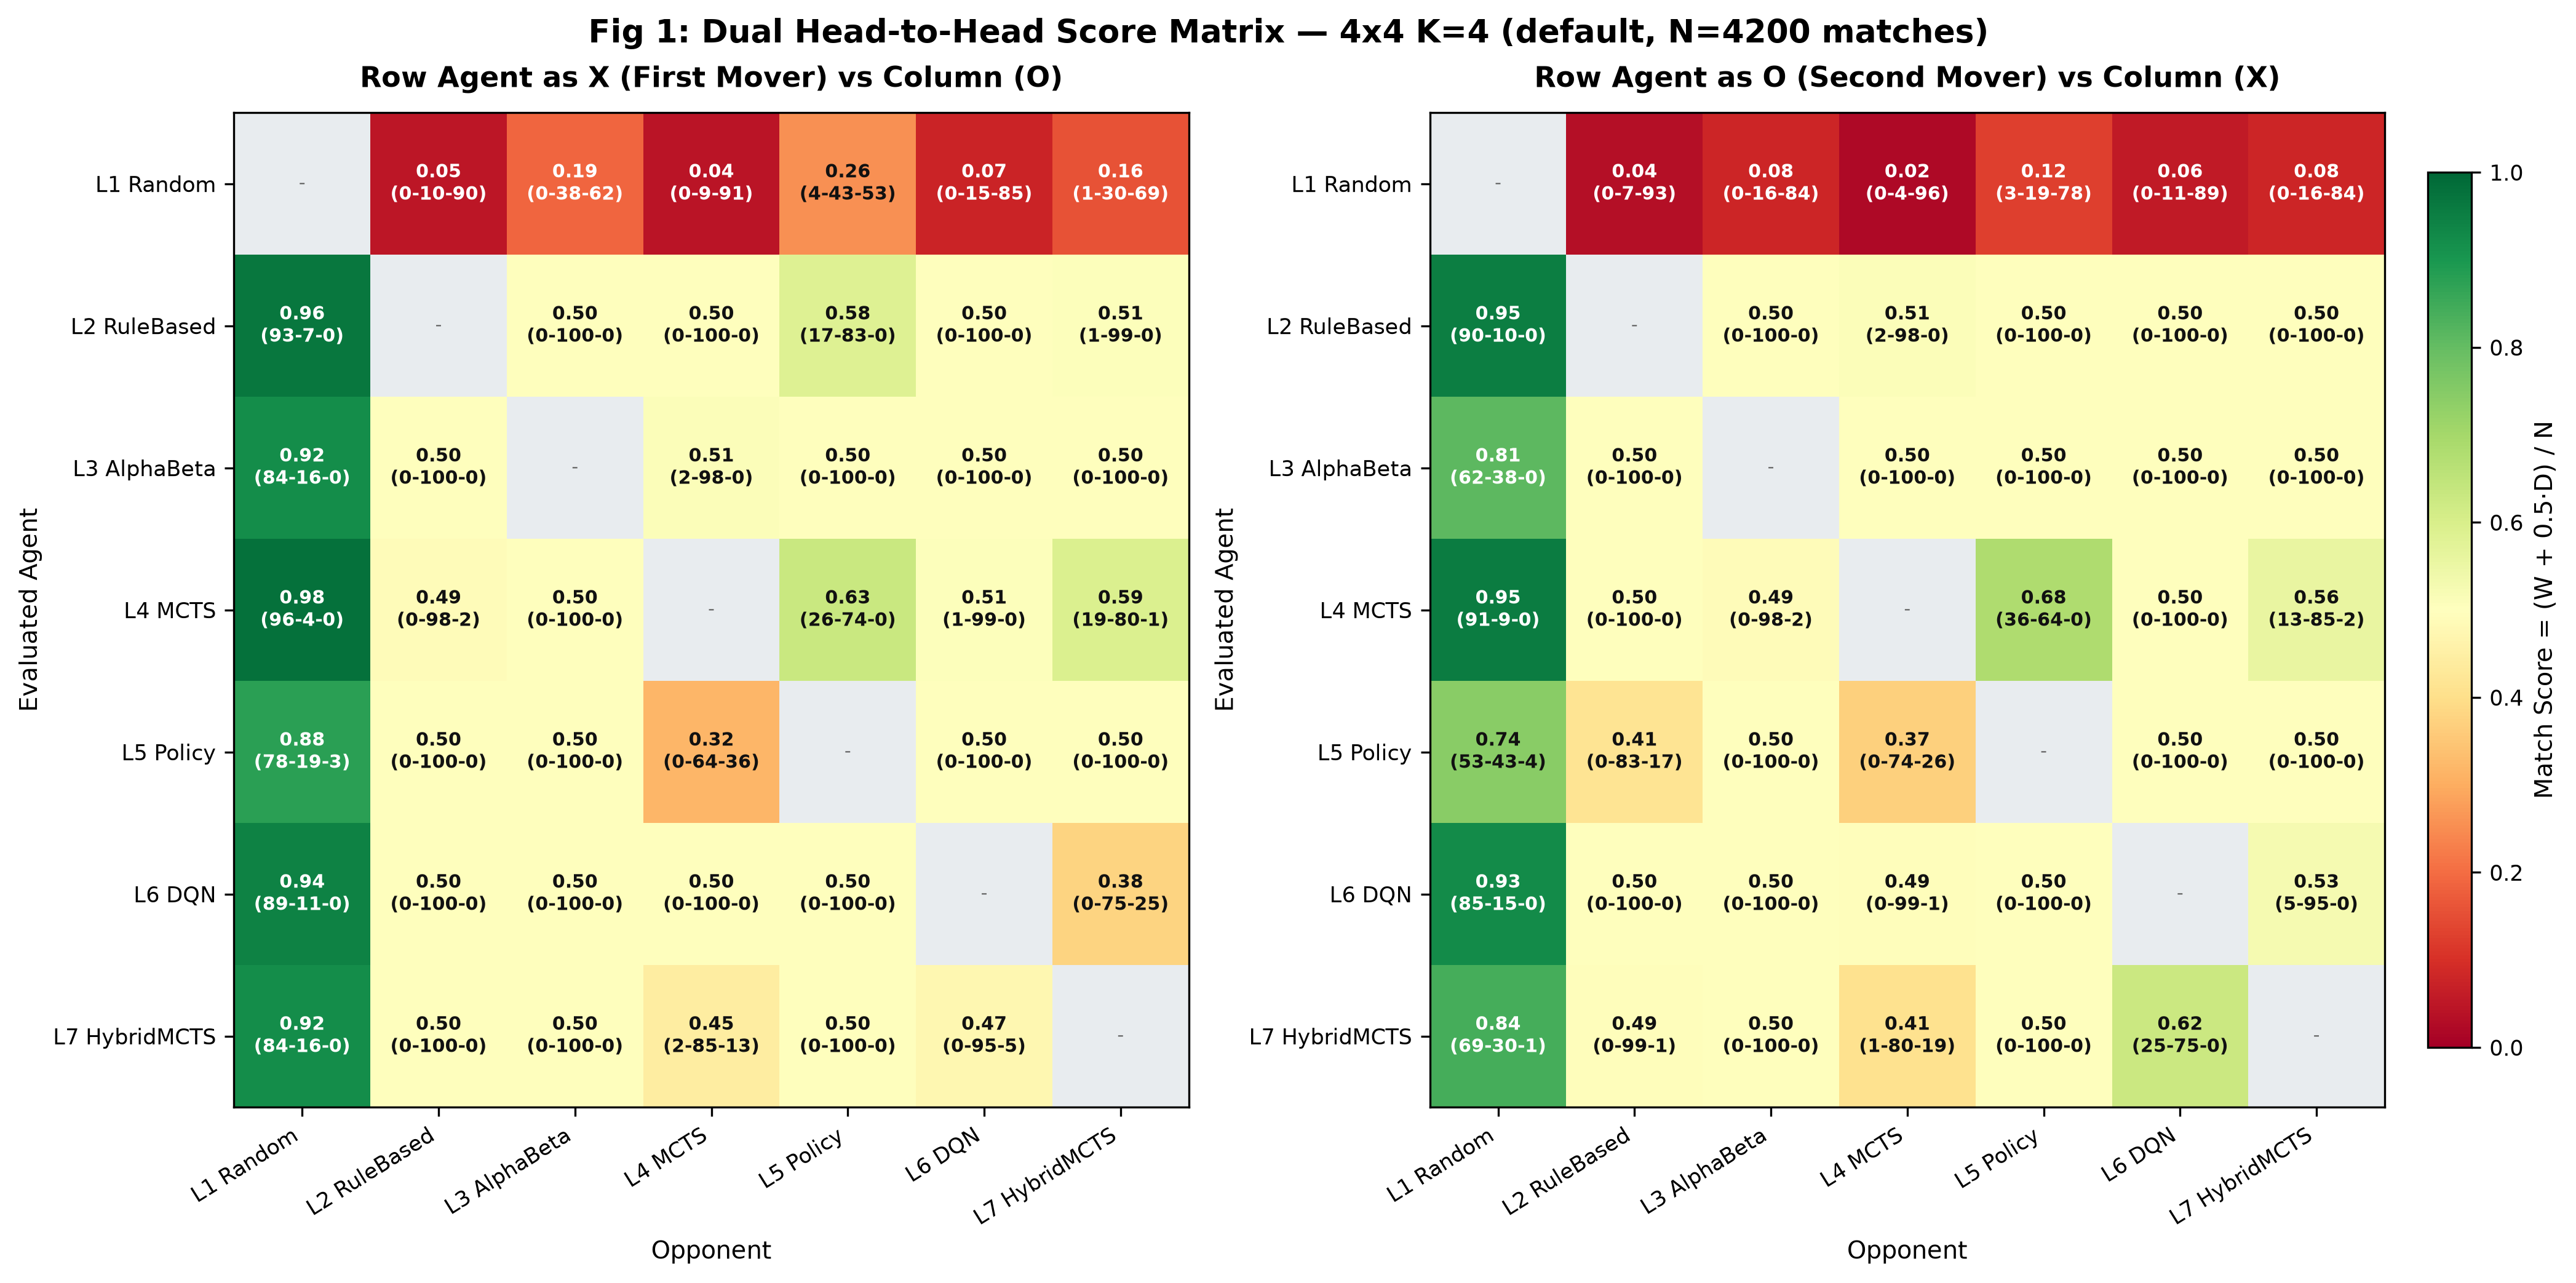
\includegraphics[width=\textwidth]{reports/figures/fig1_head_to_head_matrix.png}
    \caption{Ma trận nhiệt đối đầu kép theo vai trò đi trước ($X$) và đi sau ($O$) của 7 cấp độ AI trên chuẩn $4 \times 4, K=4$.}
    \label{fig:fig1_h2h}
\end{figure}

\begin{figure}[H]
    \centering
    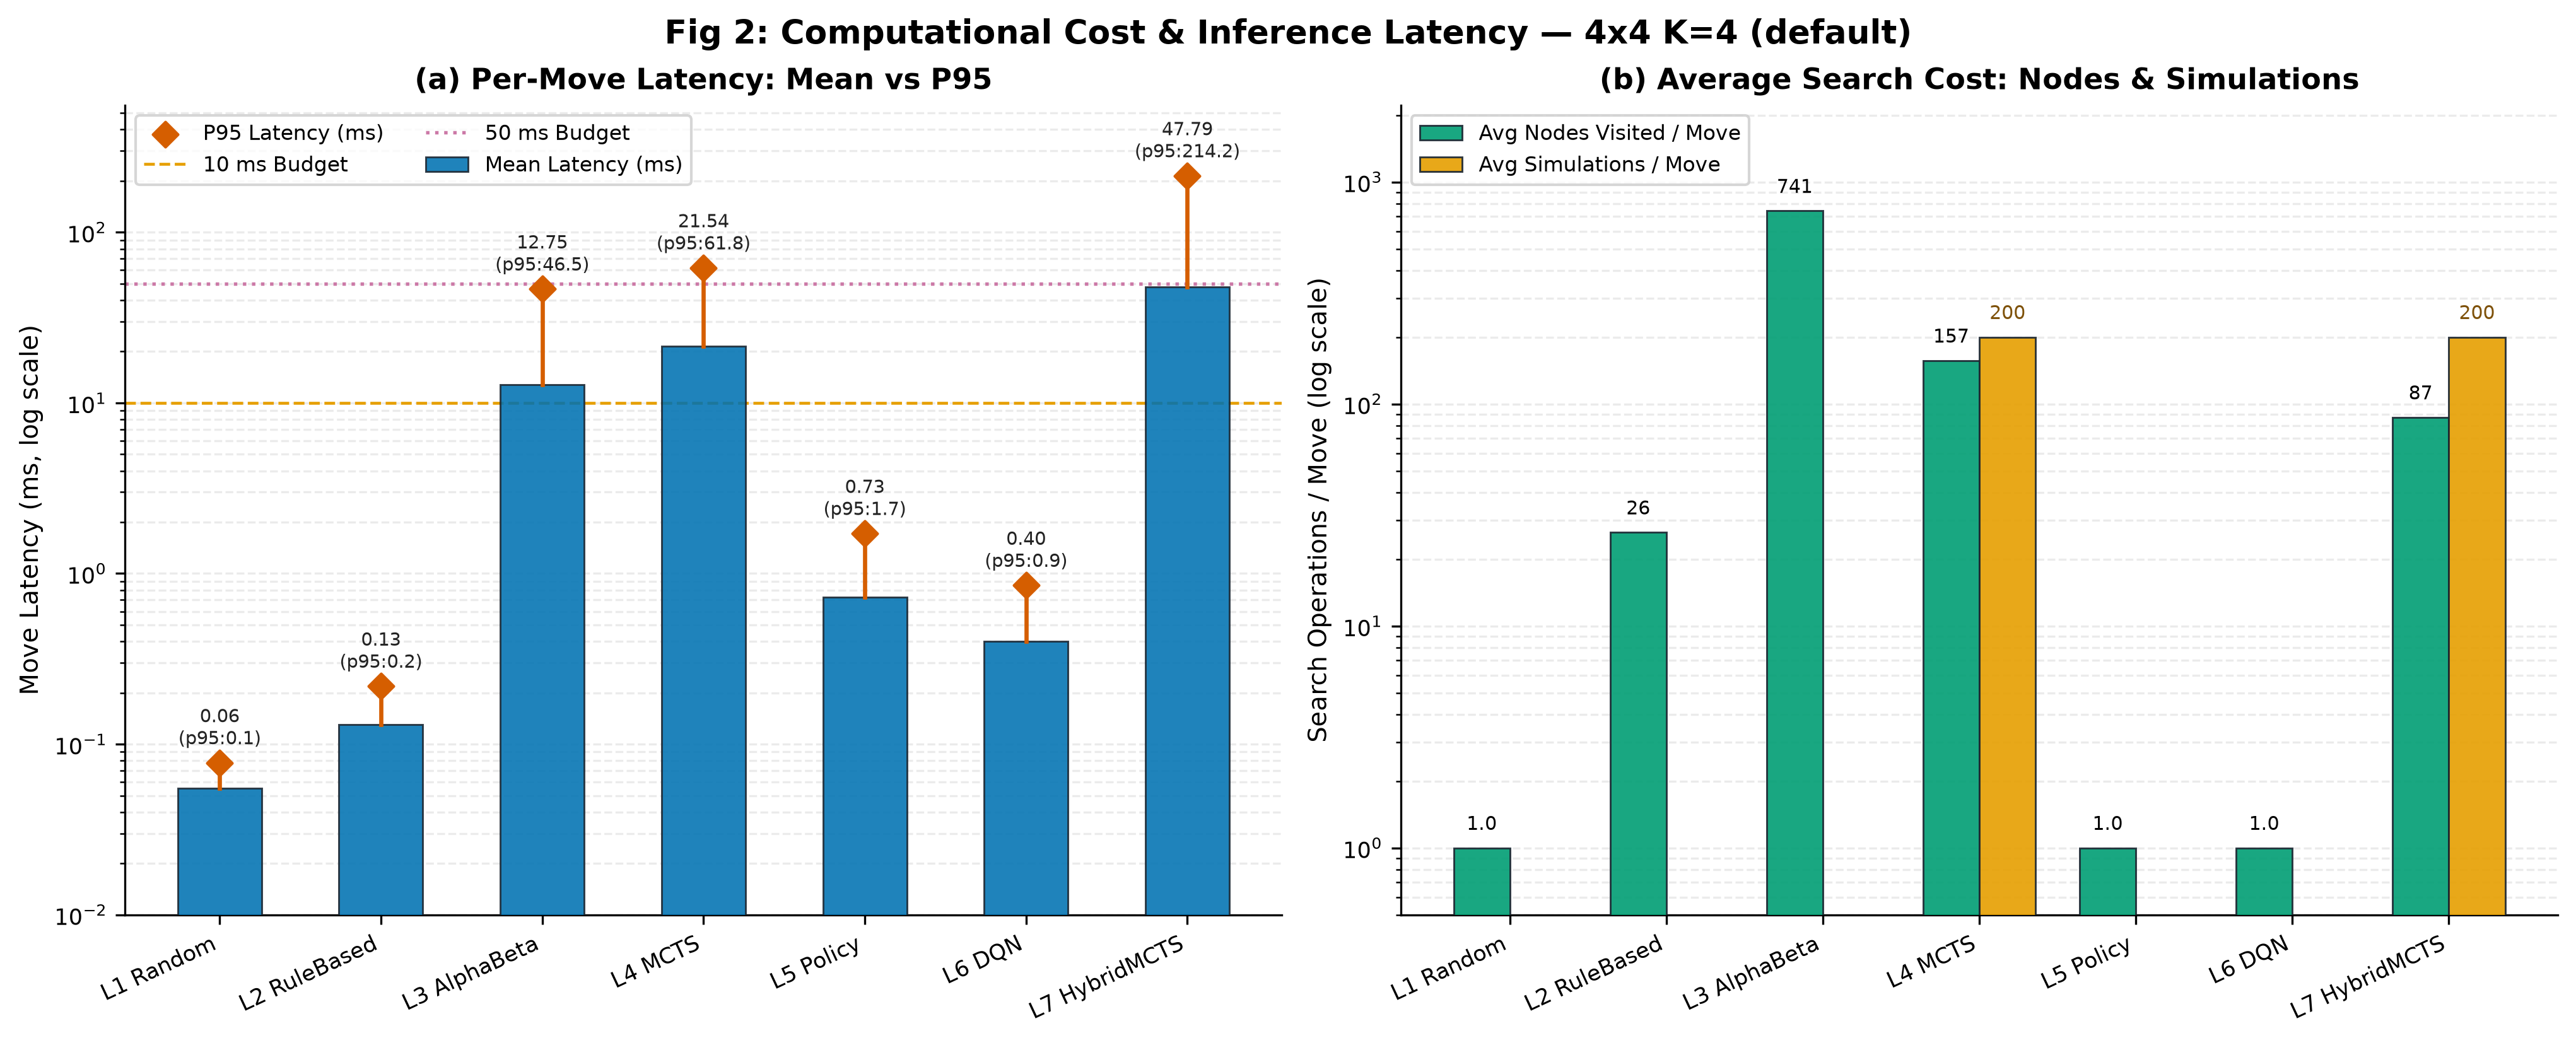
\includegraphics[width=\textwidth]{reports/figures/fig2_latency_and_nodes.png}
    \caption{Phân tích tương quan giữa độ trễ suy luận (thang logarit, gồm \texttt{mean\_ms} và \texttt{p95\_ms}) với chi phí tìm kiếm trung bình (\texttt{Avg Nodes} / \texttt{Avg Sims}).}
    \label{fig:fig2_latency}
\end{figure}

\subsection{Phân tích Thực nghiệm Trả lời 3 Câu hỏi Nghiên cứu (\texorpdfstring{$8{,}756$}{8,756} ván Ablation)}

\subsubsection{Thí nghiệm 1: Cắt tỉa Alpha-Beta và Sắp xếp Nước đi (Ablation 1 --- $316$ ván \& $12$ state probes)}
Thí nghiệm đối chứng ba biến thể cùng độ sâu $d \in \{2, 3, 4\}$ trên bàn cờ $4 \times 4, K=4$: Minimax thuần túy (\texttt{MM\_Raw}), Alpha-Beta không sắp xếp (\texttt{AB\_NoOrder}) và Alpha-Beta kết hợp Move Ordering (\texttt{AB\_Order}). Số liệu kiểm chứng cho thấy:
\begin{itemize}[leftmargin=1.2cm]
    \item Tại độ sâu $d=4$ trên $12$ trạng thái thăm dò (state probes), \texttt{MM\_Raw} phải duyệt trung bình $23{,}171.0$ nút ($211.56\text{ ms}$), \texttt{AB\_NoOrder} giảm xuống $2{,}035.5$ nút (cắt giảm $-91.22\%$), và \texttt{AB\_Order} chỉ cần duyệt \textbf{$1{,}225.0$ nút} ($11.78\text{ ms}$, \textbf{giảm $-94.71\%$}).
    \item Trong các ván đấu đối đầu thực tế ($316$ trận, độ sâu $d=4$), chi phí trung bình mỗi nước của \texttt{AB\_Order\_d4} chỉ là $805.6$ nút ($7.88\text{ ms}$, $p95 = 19.32\text{ ms}$) so với $11{,}368.8$ nút ($105.76\text{ ms}$) của \texttt{MM\_Raw\_d4} (giảm $-92.91\%$). Cả ba biến thể đều trả về \textbf{cùng một hành động và giá trị lượng giá gốc chính xác tuyệt đối} (\texttt{all\_\allowbreak exact\_\allowbreak value\_\allowbreak match=True}), khẳng định tính đúng đắn toán học của cơ chế cắt tỉa.
\end{itemize}

\subsubsection{Thí nghiệm 2: Trả lời RQ1 --- Ưu thế của Hybrid MCTS (Ablation 2 --- $2{,}760$ ván)}
Bảng~\ref{tab:abl2_rq1} tổng hợp kết quả thực nghiệm đối đầu $18$ cấu hình trên $4 \times 4, K=4$ nhằm trả lời trực tiếp câu hỏi nghiên cứu \textbf{RQ1}.

\begin{table}[H]
\centering
\footnotesize
\setlength{\tabcolsep}{4pt}
\caption{Kết quả Ablation 2 (RQ1): So sánh \texttt{Policy-only}, \texttt{Pure MCTS} và \texttt{Hybrid MCTS} trên $4 \times 4, K=4$ ($2{,}760$ ván)}
\label{tab:abl2_rq1}
\vspace{0.2cm}
\begin{tabular}{p{3.8cm}ccrrr}
\toprule
\textbf{Ứng viên} & \textbf{Ngân sách} & \textbf{Score [95\% CI]} & \textbf{Mean (ms)} & \textbf{Avg Sims} & \textbf{Cache Hit} \\
\midrule
\texttt{Policy\_\allowbreak Fast} & Không tìm kiếm & 0.542 [0.496, 0.588] & 0.35 & 0.0 & -- \\
\texttt{Policy\_\allowbreak Strong} & Không tìm kiếm & 0.525 [0.479, 0.575] & 0.34 & 0.0 & -- \\
\texttt{Value\_\allowbreak Greedy} & Không tìm kiếm & 0.296 [0.225, 0.371] & 0.43 & 0.0 & -- \\
\midrule
\texttt{PureMCTS\_\allowbreak sim50} & 50 sims & 0.529 [0.471, 0.588] & 3.79 & 50.0 & -- \\
\texttt{HybridRollout\_\allowbreak sim50} & 50 sims & \textbf{0.583 [0.542, 0.625]} & 8.78 & 50.0 & 47.0\% \\
\texttt{HybridMixed\_\allowbreak sim50} & 50 sims & 0.575 [0.533, 0.621] & 8.99 & 50.0 & 60.7\% \\
\midrule
\texttt{PureMCTS\_\allowbreak sim150} & 150 sims & 0.604 [0.571, 0.642] & 10.75 & 150.0 & -- \\
\texttt{HybridRollout\_\allowbreak sim150} & 150 sims & 0.579 [0.537, 0.621] & 22.81 & 150.0 & 47.3\% \\
\texttt{HybridMixed\_\allowbreak sim150} & 150 sims & 0.567 [0.521, 0.613] & 23.67 & 150.0 & 63.9\% \\
\midrule
\texttt{PureMCTS\_\allowbreak sim400} & 400 sims & \textbf{0.621 [0.583, 0.658]} & 28.51 & 400.0 & -- \\
\texttt{HybridRollout\_\allowbreak sim400} & 400 sims & 0.558 [0.521, 0.596] & 55.24 & 400.0 & 47.1\% \\
\texttt{HybridMixed\_\allowbreak sim400} & 400 sims & 0.600 [0.562, 0.637] & 56.74 & 400.0 & 62.8\% \\
\midrule
\texttt{PureMCTS\_\allowbreak time10ms} & $10.0\text{ ms}$ & 0.613 [0.571, 0.654] & 9.27 & 190.7 & -- \\
\texttt{HybridRollout\_\allowbreak time10ms} & $10.0\text{ ms}$ & 0.575 [0.533, 0.617] & 9.41 & 144.0 & 51.2\% \\
\texttt{HybridMixed\_\allowbreak time10ms} & $10.0\text{ ms}$ & 0.583 [0.542, 0.625] & 9.47 & 145.9 & 68.7\% \\
\midrule
\texttt{PureMCTS\_\allowbreak time50ms} & $50.0\text{ ms}$ & 0.608 [0.571, 0.646] & 28.49 & 396.8 & -- \\
\texttt{HybridRollout\_\allowbreak time50ms} & $50.0\text{ ms}$ & 0.583 [0.542, 0.625] & 33.38 & 313.2 & 52.1\% \\
\texttt{HybridMixed\_\allowbreak time50ms} & $50.0\text{ ms}$ & 0.579 [0.533, 0.625] & 34.04 & 312.1 & 69.0\% \\
\bottomrule
\end{tabular}
\end{table}

\textbf{Kết luận cho RQ1:}
\begin{itemize}[leftmargin=1.2cm]
    \item \textbf{Tại ngân sách mô phỏng thấp ($N_{\text{sims}} = 50$):} Giả thuyết được xác nhận hoàn toàn. \texttt{Hybrid\_\allowbreak Rollout} đạt Score $0.583$ $[0.542, 0.625]$ (chỉ thua $5$ ván) và \texttt{Hybrid\_\allowbreak Mixed} đạt $0.575$ $[0.533, 0.621]$ (với độ sâu cây tìm kiếm trung bình đạt tới $6.46$ tầng), vượt trội rõ rệt so với \texttt{Pure\_\allowbreak MCTS\_\allowbreak sim50} (Score $0.529$, thua tới $22$ ván, độ sâu trung bình chỉ đạt $2.42$ tầng) và \texttt{Policy\_\allowbreak Strong} thuần không duyệt cây (Score $0.525$, thua $14$ ván). Tri thức tiên nghiệm $P(s, a)$ giúp PUCT đào sâu ngay vào các nhánh chiến thuật trọng yếu thay vì tiêu phí ngân sách cho mở rộng bề ngang ngẫu nhiên.
    \item \textbf{Tại ngân sách cao ($N_{\text{sims}} = 400$ và giới hạn $10 / 50\text{ ms}$):} Trên không gian có chiều sâu nhánh không quá lớn ($4 \times 4$), \texttt{Pure\_\allowbreak MCTS} vươn lên đạt Score $0.621$ ở mốc $400$ simulations nhờ chi phí mỗi lần rollout cực thấp ($28.51\text{ ms}$), trong khi \texttt{Hybrid\_\allowbreak Mixed} tiêu tốn $56.74\text{ ms}$ do chi phí suy luận PyTorch trên CPU (mặc dù LRU Cache đã hấp thụ thành công $62.8\%$--$69.0\%$ số lần gọi mạng). Dưới ràng buộc thời gian thực $10\text{ ms}$, \texttt{Pure\_\allowbreak MCTS} thực hiện được nhiều hơn khoảng $31\%$ số lượt mô phỏng ($190.7$ so với $145.9$ sims của Hybrid), tạo ra sự đánh đổi rõ rệt giữa \textit{hiệu suất trên mỗi lượt mô phỏng} (Hybrid thắng thế ở $N_{\text{sims}}$ nhỏ) và \textit{tốc độ thô trên mỗi mili-giây} (Pure MCTS thắng thế trên bàn cờ nhẹ).
\end{itemize}

Hình~\ref{fig:fig3_rq1} minh họa đồng thời đường cong hiệu năng theo ngân sách của Ablation 2 (RQ1) và hiệu quả cắt giảm nút duyệt của Ablation 1.

\begin{figure}[H]
    \centering
    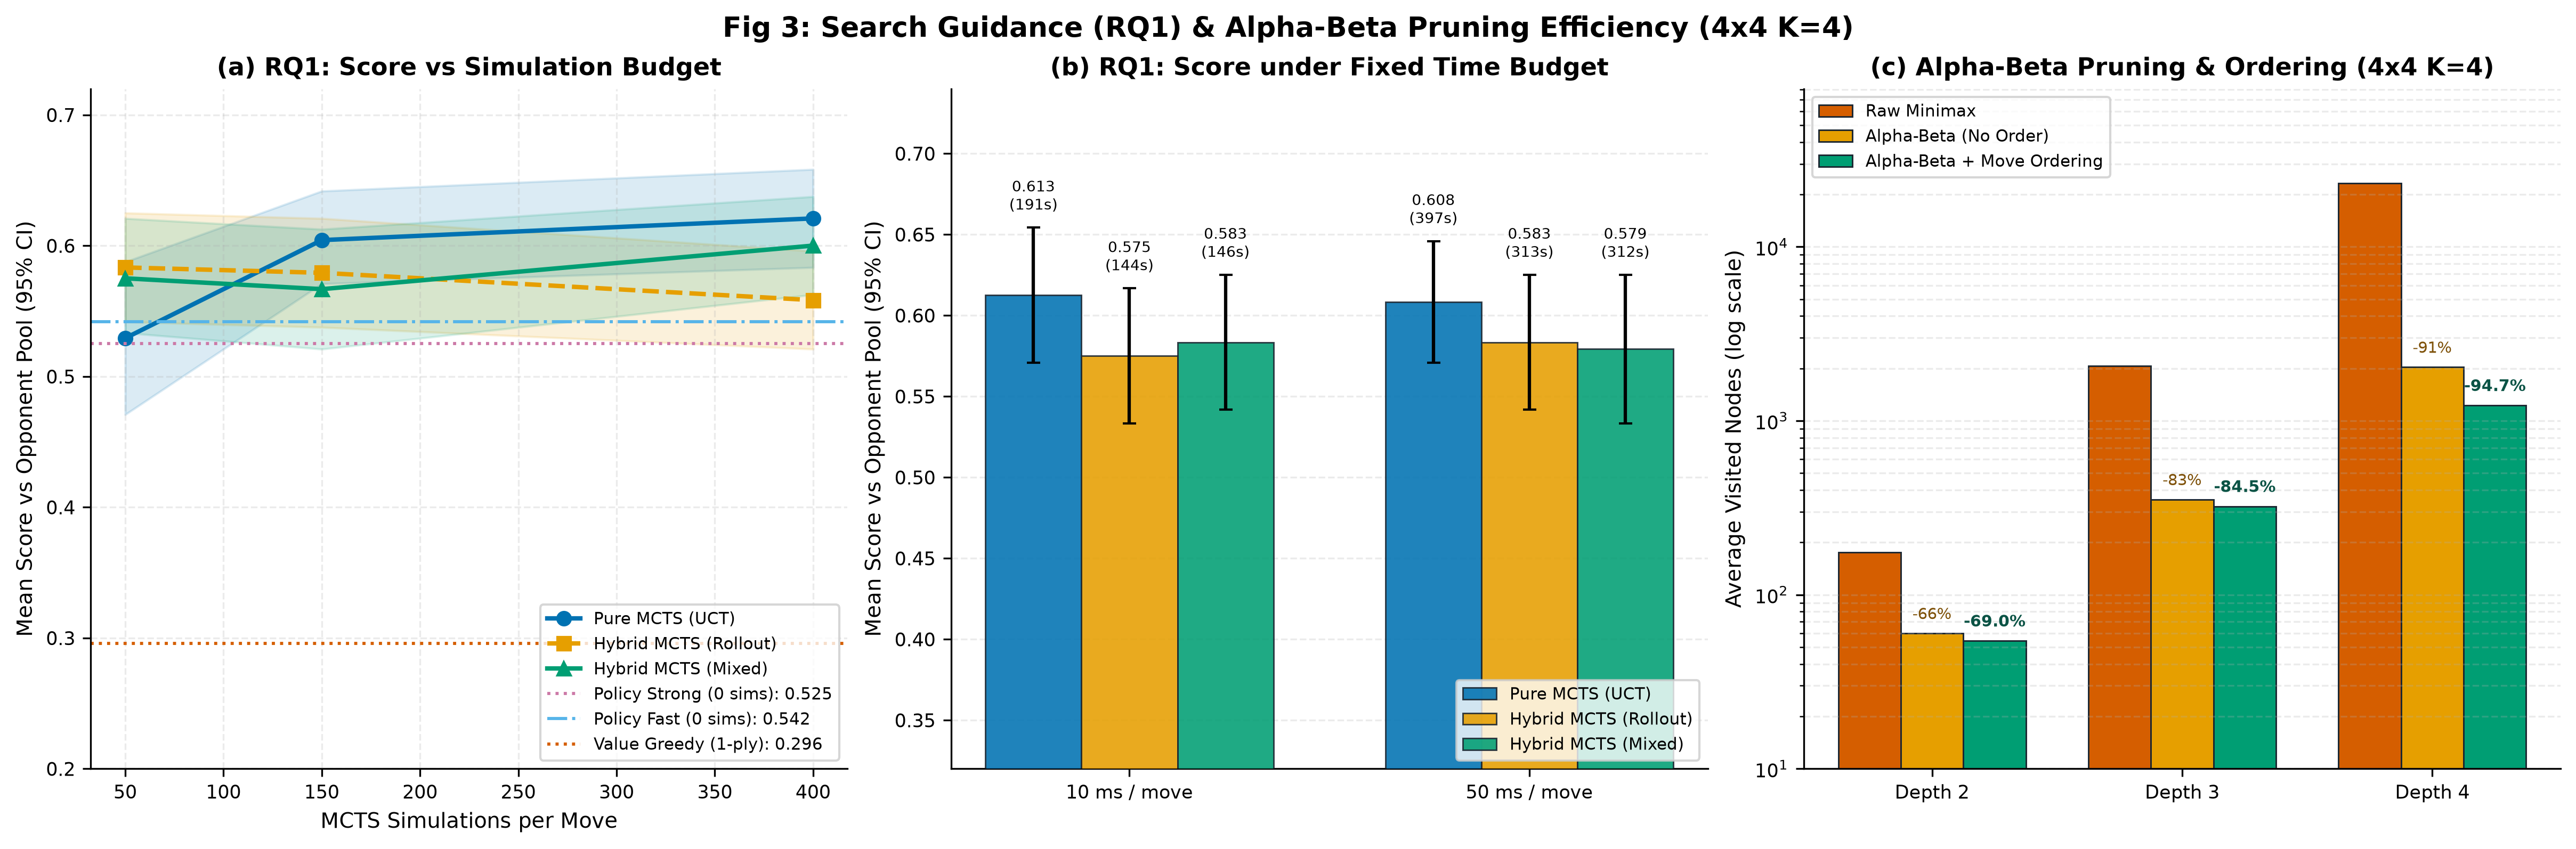
\includegraphics[width=\textwidth]{reports/figures/fig3_ablation_rq1_and_alphabeta.png}
    \caption{Kết quả thực nghiệm trả lời RQ1 (\texttt{Policy-only} vs. \texttt{Pure MCTS} vs. \texttt{Hybrid MCTS} theo số mô phỏng và ngưỡng thời gian) cùng tỷ lệ cắt giảm nút của Alpha-Beta Pruning.}
    \label{fig:fig3_rq1}
\end{figure}

\subsubsection{Thí nghiệm 3: Trả lời RQ2 --- Lợi thế Người Đi Trước $\Delta\text{Score}$ (Ablation 3 --- $2{,}080$ ván)}
Bảng~\ref{tab:abl3_rq2} tổng hợp sự dịch chuyển cán cân thắng/hòa và lợi thế đi trước giữa ba cấu hình luật thắng trên tổng số $2{,}080$ ván đấu.

\begin{table}[H]
\centering
\small
\setlength{\tabcolsep}{6pt}
\caption{Kết quả Ablation 3 (RQ2): So sánh lợi thế người đi trước ($\Delta\text{Score}$) theo cấu hình bàn cờ}
\label{tab:abl3_rq2}
\vspace{0.2cm}
\begin{tabular}{lrrrrl}
\toprule 
\textbf{Cấu hình bàn cờ} & \textbf{Số ván} & \textbf{X Thắng} & \textbf{Hòa} & \textbf{O Thắng} & \textbf{$\Delta\text{Score} = \text{Score}_X - \text{Score}_O$} \\ 
& & & & & \textbf{[95\% CI]} \\
\midrule
$4 \times 4, K=3$ & 400 & 76.5\% & 0.0\% & 23.5\% & $+0.530$ $[+0.445, +0.610]$ \\
$3 \times 3, K=3$ & 840 & 23.8\% & 63.6\% & 12.6\% & $+0.112$ $[+0.073, +0.152]$ \\
$4 \times 4, K=4$ & 840 & 14.2\% & 74.1\% & 11.8\% & $+0.024$ $[-0.011, +0.058]$ \\
\bottomrule
\end{tabular}
\end{table}

\textbf{Kết luận cho RQ2:}
\begin{itemize}[leftmargin=1.2cm]
    \item \textbf{Sự bùng nổ cực đoan trên $4 \times 4, K=3$:} Khi bàn cờ rộng $16$ ô nhưng chỉ cần $3$ quân thẳng hàng để thắng, ván đấu hoàn toàn mất khả năng thủ hòa ($0.0\%$ hòa). Quân đi trước $X$ giành chiến thắng tới $76.5\%$, tạo ra chênh lệch khổng lồ $\Delta\text{Score} = +0.530$ $[0.445, 0.610]$. Đặc biệt, mọi tác tử có năng lực chiến thuật (\texttt{RuleBased}, \texttt{AlphaBeta}, \texttt{DQN}) khi cầm quân $X$ đều đạt tỷ lệ thắng tuyệt đối \textbf{$100\%$ ($\text{Score}_X = 1.000$)}.
    \item \textbf{Chế độ đối chứng $3 \times 3, K=3$:} Tỷ lệ hòa đạt $63.6\%$ với $\Delta\text{Score} = +0.112$ $[0.073, 0.152]$, chủ yếu do các tác tử mạnh dễ dàng trừng phạt lỗi mở màn khi cầm $X$ trước \texttt{Random} và \texttt{StrongPolicy}.
    \item \textbf{Sự cân bằng trên chuẩn chính $4 \times 4, K=4$:} Nâng điều kiện thắng lên $K=4$ giúp không gian phòng thủ trở nên rộng rãi, đẩy tỷ lệ hòa lên $74.1\%$ ($X$ thắng $14.2\%$, $O$ thắng $11.8\%$) và kéo lợi thế người đi trước sụp đổ về sát điểm cân bằng: $\Delta\text{Score} = +0.024$ $[-0.011, +0.058]$ (khoảng tin cậy 95\% chứa giá trị $0$). Điều này khẳng định tính hợp lý của việc lựa chọn $4 \times 4, K=4$ làm thước đo chính cho năng lực chiến thuật thuần túy của các AI.
\end{itemize}

\begin{figure}[H]
    \centering
    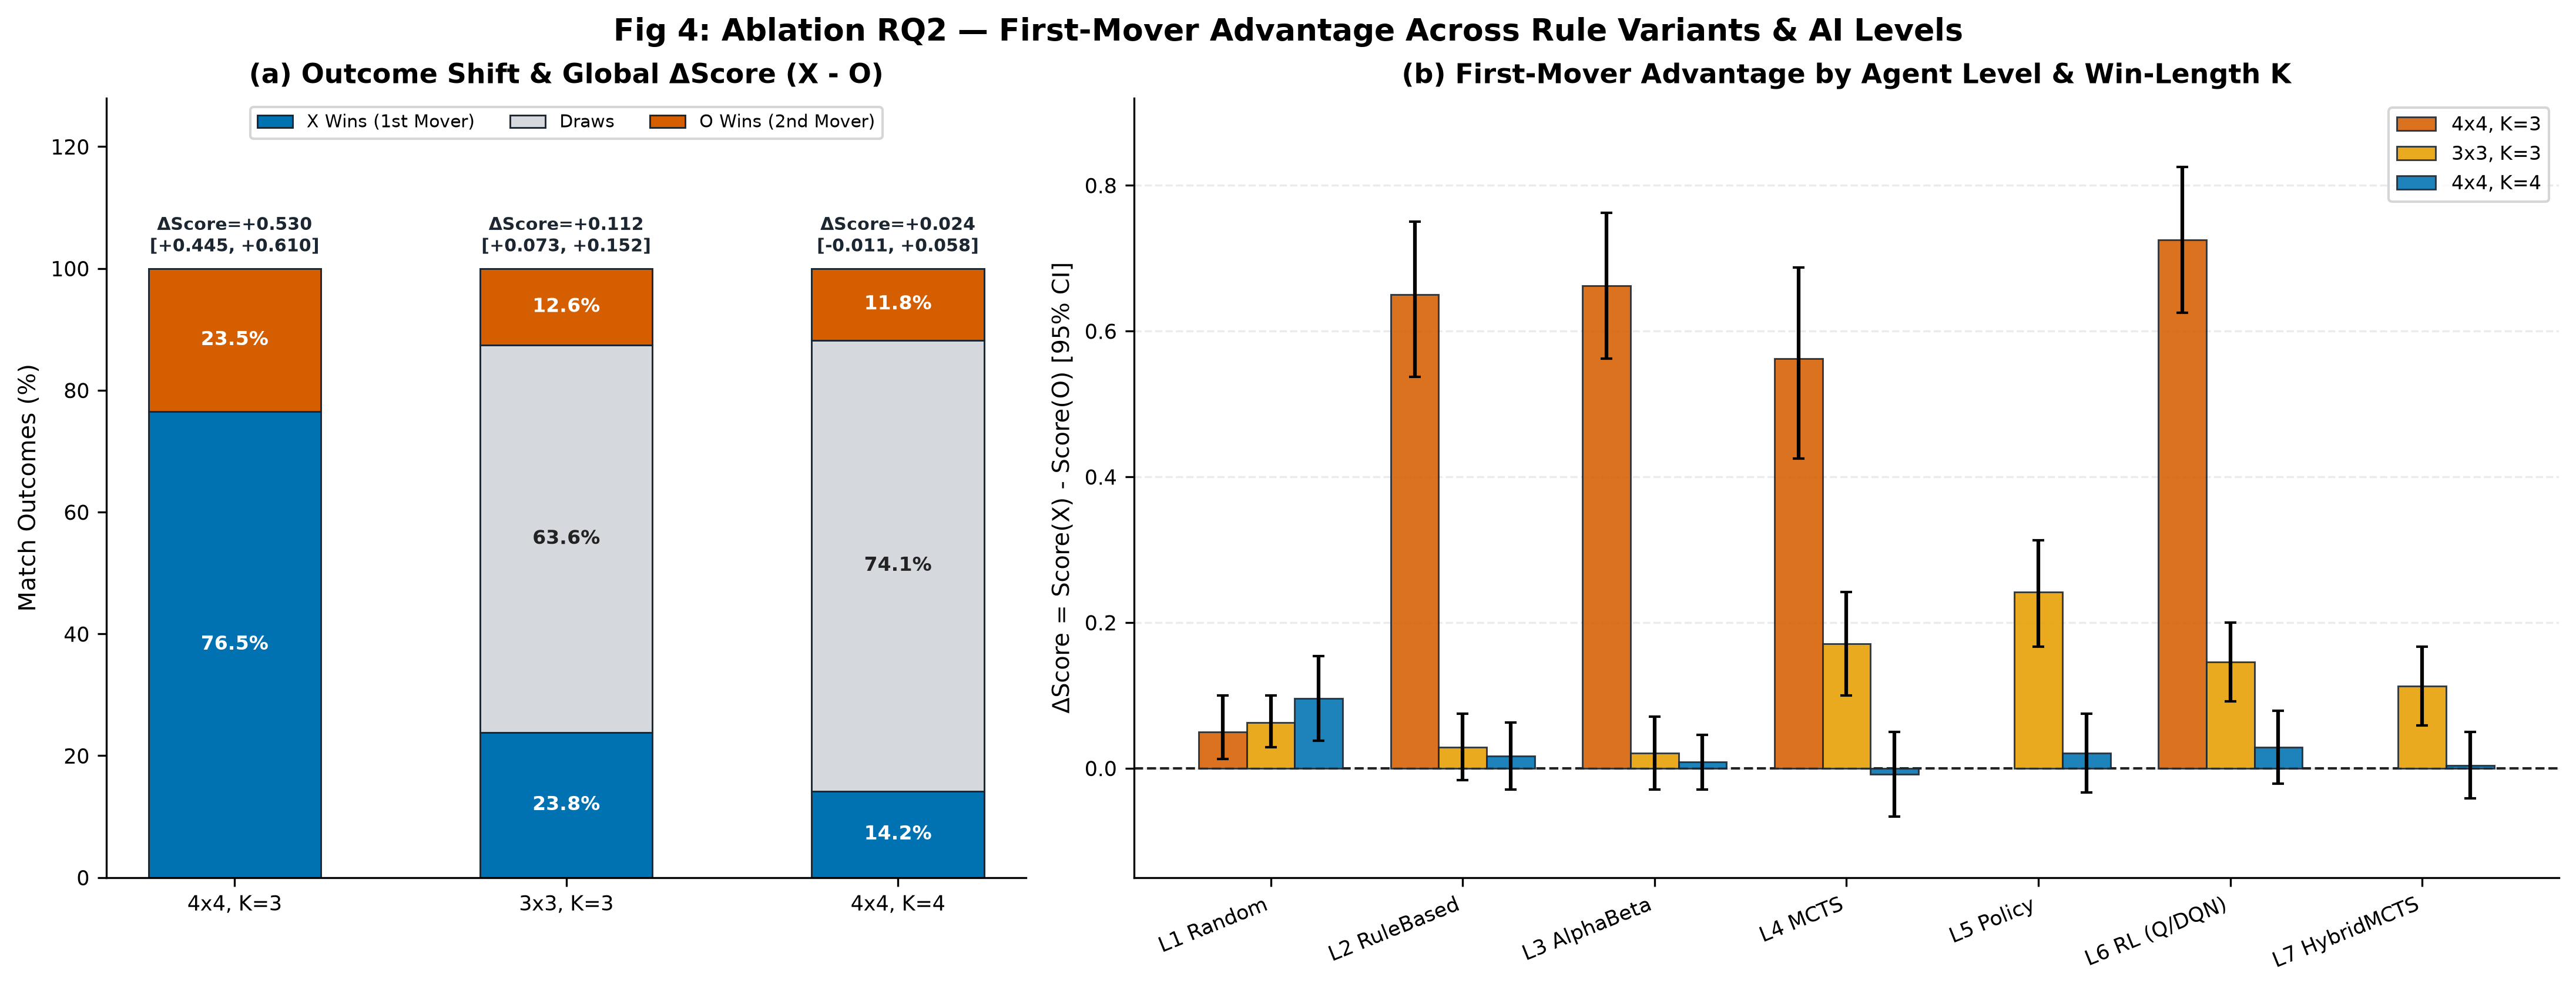
\includegraphics[width=\textwidth]{reports/figures/fig4_ablation_rq2_seat_advantage.png}
    \caption{Phân tích dịch chuyển tỷ lệ Thắng/Hòa/Thua theo ghế ($X$ vs $O$) và độ chênh lệch $\Delta\text{Score}$ trên các cấu hình $4\times 4, K=3$, $3\times 3, K=3$ và $4\times 4, K=4$ (RQ2).}
    \label{fig:fig4_rq2}
\end{figure}

\subsubsection{Thí nghiệm 4: Trả lời RQ3 --- Độ Ổn định RL Self-Play vs. Supervised (Ablation 4 --- $3{,}600$ ván)}
Thí nghiệm 4 kiểm chứng trực tiếp khả năng tổng quát hóa của các mô hình học được qua $3$ random seeds (`42, 123, 999`) khi đối đầu tập đối thủ chưa từng gặp trong lúc huấn luyện (unseen opponents gồm \texttt{MCTS} và \texttt{AlphaBeta} giới hạn độ sâu).

\begin{table}[H]
\centering
\footnotesize
\setlength{\tabcolsep}{4pt}
\caption{Kết quả Ablation 4 (RQ3): Độ ổn định và tổng quát hóa trước đối thủ Unseen ($3{,}600$ ván)}
\label{tab:abl4_rq3}
\vspace{0.2cm}
\begin{tabular}{llccccr}
\toprule
\textbf{Bàn cờ} & \textbf{Ứng viên} & \textbf{Nhóm} & \textbf{Score} & \textbf{vs Unseen} & \textbf{vs Unseen} & \textbf{Mean} \\
 & & & \textbf{Chung} & \textbf{MCTS} & \textbf{All} & \textbf{(ms)} \\
\midrule
$4\times 4, K=4$ & \texttt{SL\_\allowbreak FastPolicy} & Supervised & 0.514 & 0.425 & 0.463 & 0.32 \\
$4\times 4, K=4$ & \texttt{SL\_\allowbreak StrongPolicy} & Supervised & 0.497 & 0.344 & 0.422 & 0.35 \\
$4\times 4, K=4$ & \texttt{SL\_\allowbreak ValueGreedy} & Supervised & 0.307 & 0.256 & 0.253 & 0.45 \\
\cmidrule(lr){2-7}
$4\times 4, K=4$ & \texttt{RL\_\allowbreak DQN\_\allowbreak seed42} & RL & 0.582 & 0.537 & 0.519 & 0.26 \\
$4\times 4, K=4$ & \texttt{RL\_\allowbreak DQN\_\allowbreak seed123} & RL & 0.621 & 0.575 & 0.537 & 0.23 \\
$4\times 4, K=4$ & \texttt{RL\_\allowbreak DQN\_\allowbreak seed999} & RL & 0.556 & 0.550 & 0.525 & 0.23 \\
\midrule
$3\times 3, K=3$ & \texttt{SL\_\allowbreak FastPolicy} & Supervised & 0.476 & 0.556 & 0.528 & 0.24 \\
$3\times 3, K=3$ & \texttt{SL\_\allowbreak StrongPolicy} & Supervised & 0.485 & 0.581 & 0.541 & 0.25 \\
$3\times 3, K=3$ & \texttt{SL\_\allowbreak ValueGreedy} & Supervised & 0.469 & 0.506 & 0.503 & 0.29 \\
\cmidrule(lr){2-7}
$3\times 3, K=3$ & \texttt{RL\_\allowbreak TabQ\_\allowbreak seed42} & RL & 0.653 & 0.594 & 0.547 & 0.03 \\
$3\times 3, K=3$ & \texttt{RL\_\allowbreak TabQ\_\allowbreak seed123} & RL & 0.661 & 0.613 & 0.556 & 0.03 \\
$3\times 3, K=3$ & \texttt{RL\_\allowbreak TabQ\_\allowbreak seed999} & RL & 0.664 & 0.650 & 0.575 & 0.03 \\
\bottomrule
\end{tabular}
\end{table}

\textbf{Kết luận cho RQ3:}
\begin{itemize}[leftmargin=1.2cm]
    \item \textbf{Trên $4 \times 4, K=4$:} Tác tử RL (\texttt{DQN}) qua 3 seeds (`42, 123, 999`) duy trì độ ổn định vượt trội với Score tổng thể trung bình $0.586 \pm 0.027$. Đặc biệt, khi đối đầu trực tiếp với đối thủ unseen \texttt{MCTS}, \texttt{DQN} đạt Score $0.554 \pm 0.016$ (chỉ để thua $0$--$2$ ván trên $80$ ván mỗi seed). Ngược lại, các mô hình Supervised bắt chước chuyên gia sụp đổ nặng nề trước đối thủ unseen \texttt{MCTS}: \texttt{SL\_\allowbreak StrongPolicy} tụt xuống chỉ còn $0.344$ (thua tới $27$ ván) và \texttt{SL\_\allowbreak FastPolicy} đạt $0.425$.
    \item \textbf{Trên $3 \times 3, K=3$:} \texttt{TabularQ} qua 3 seeds đạt độ ổn định gần như tuyệt đối với Score $0.659 \pm 0.005$ (vs. Unseen \texttt{MCTS} đạt $0.619 \pm 0.023$, chỉ thua $0$--$1$ ván trên $360$ trận), bỏ xa toàn bộ nhóm Supervised ($0.469$--$0.485$) và thắng trực tiếp nhóm Supervised với tỷ số áp đảo $0.750$ vs. $0.250$ ($20-20-0$) trên toàn bộ $9/9$ cặp đối đầu.
\end{itemize}

\begin{figure}[H]
    \centering
    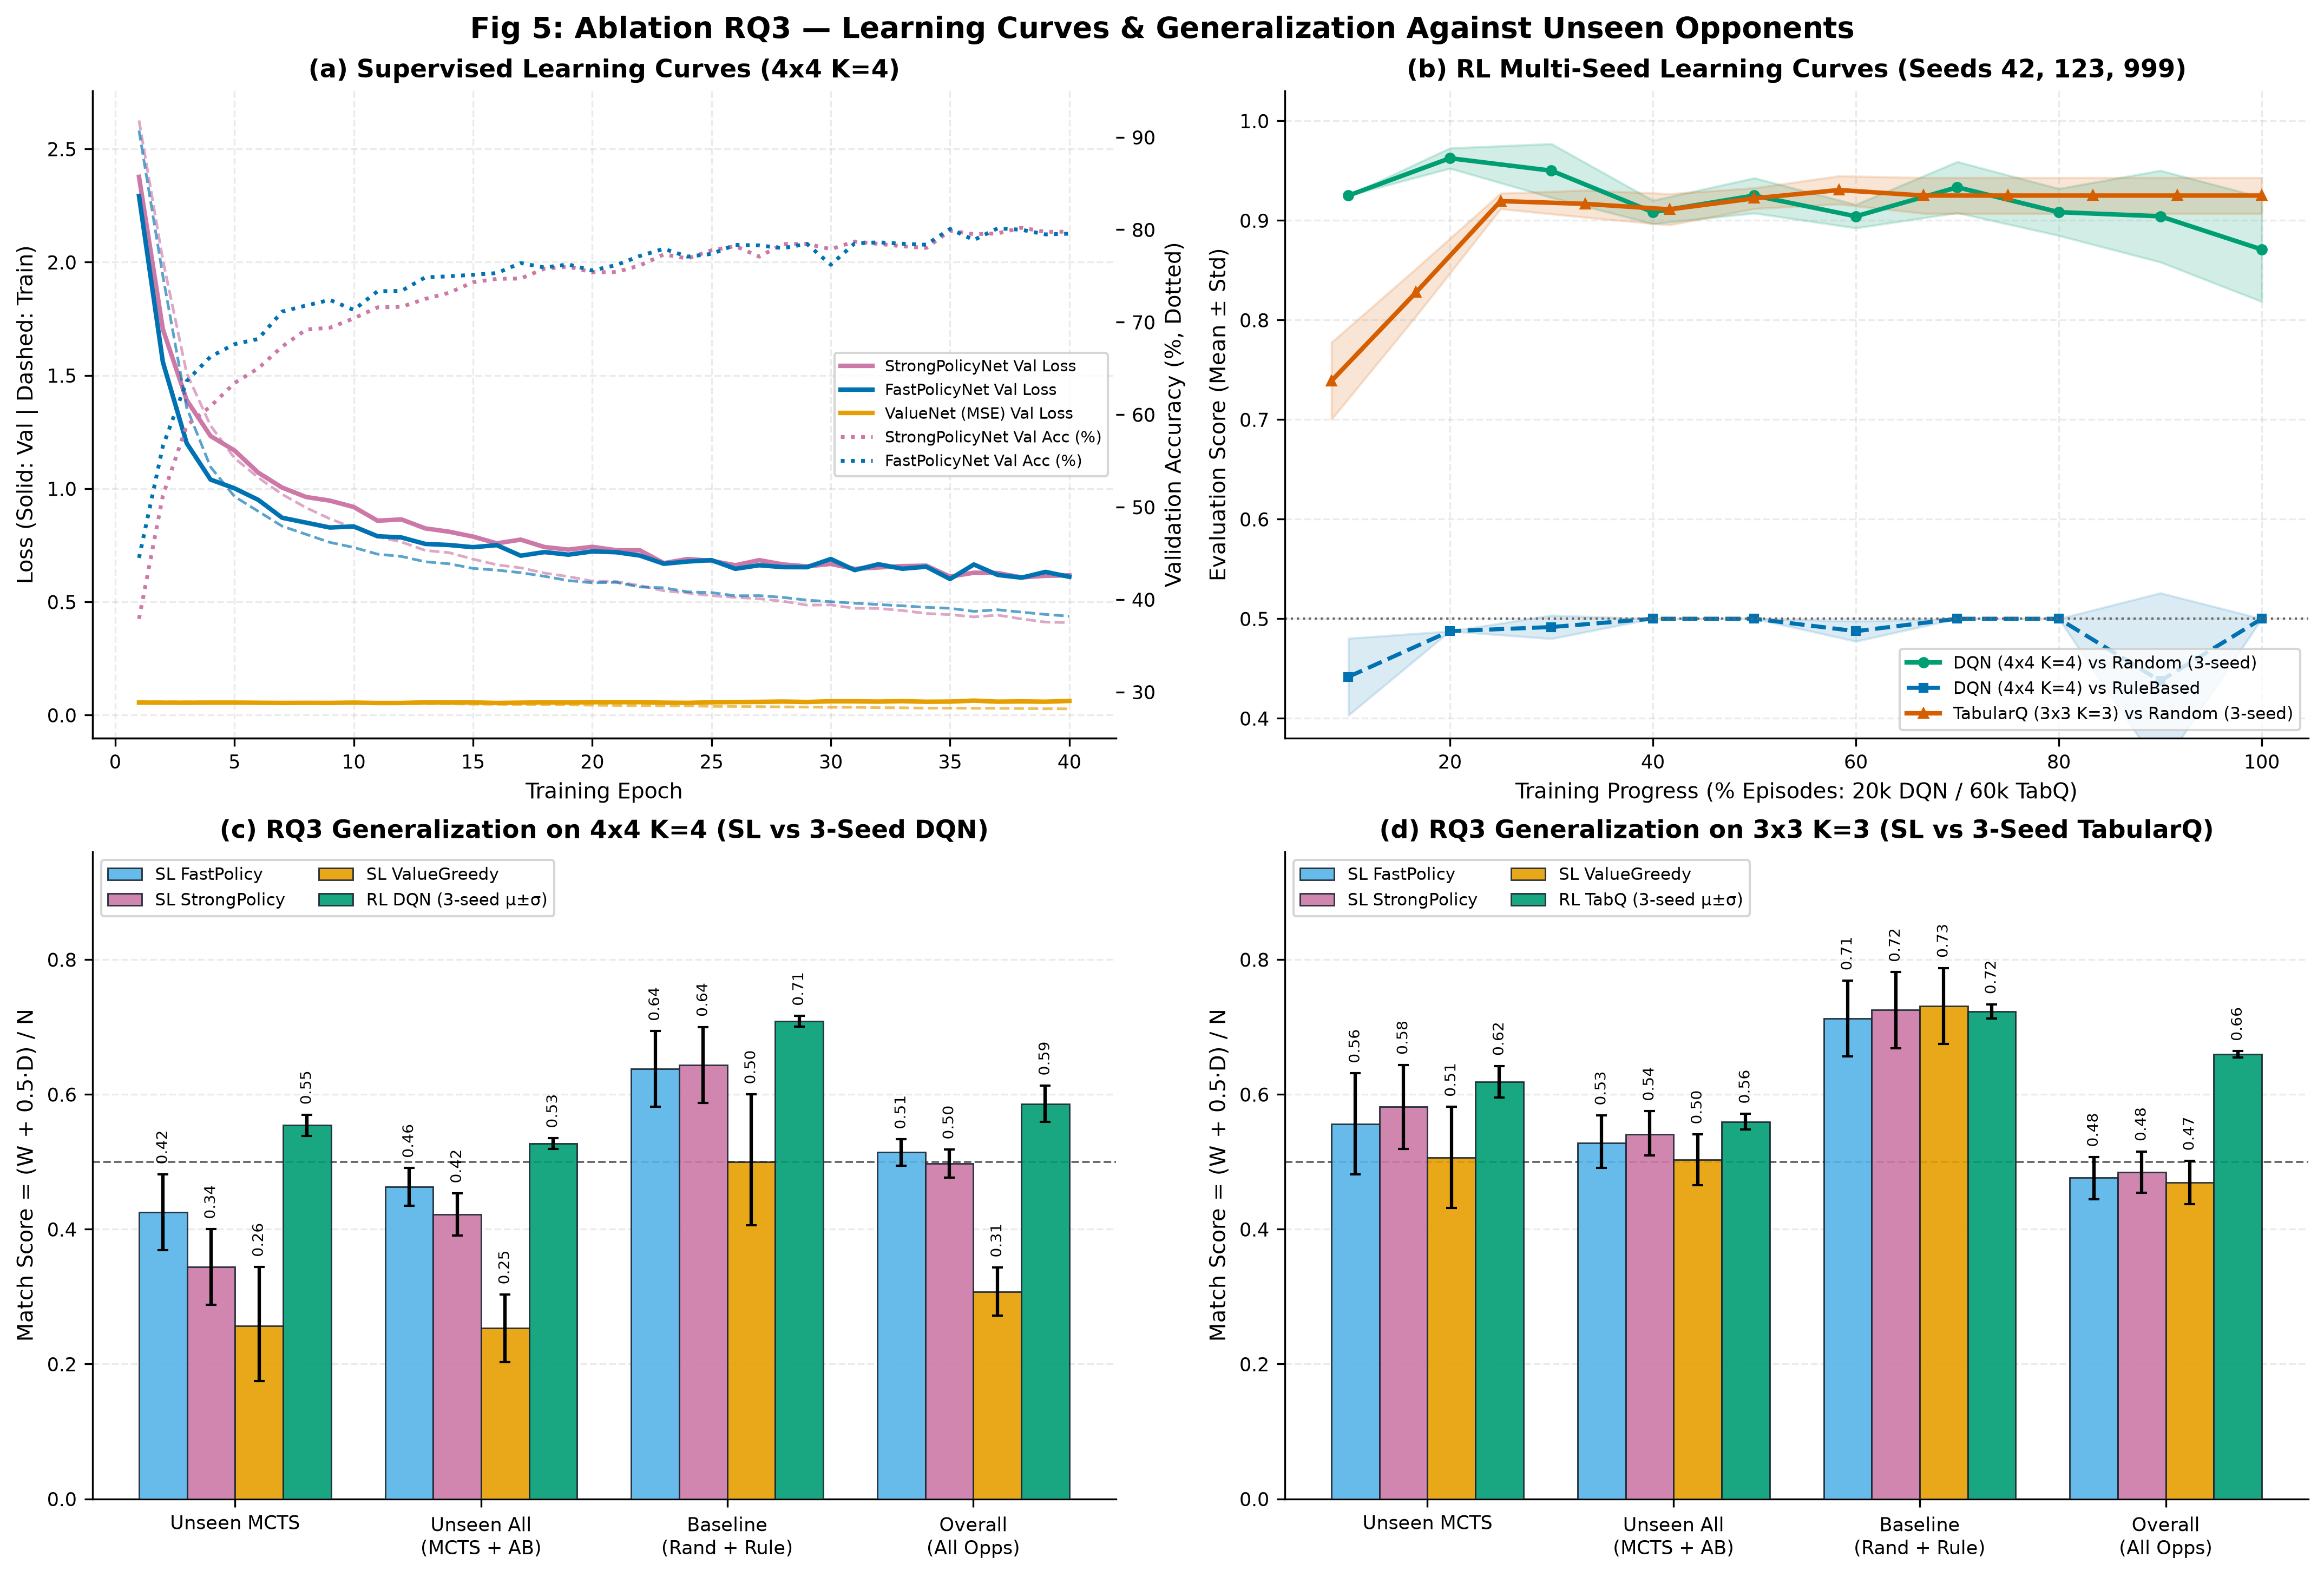
\includegraphics[width=\textwidth]{reports/figures/fig5_ablation_rq3_learning_and_generalization.png}
    \caption{Đường cong học tập đa seed của Supervised Learning và Reinforcement Learning (Tabular Q / DQN Self-Play) cùng hiệu năng tổng quát hóa trước đối thủ chưa từng gặp (RQ3).}
    \label{fig:fig5_rq3}
\end{figure}

% ==============================================================================
% CHƯƠNG 5: GIAO DIỆN RICH CLI, PHÂN TÍCH LỖI & THẢO LUẬN
% ==============================================================================
\clearpage
\section{Giao diện Rich CLI, Phân tích Lỗi \& Thảo luận}

\subsection{Thiết kế Giao diện Rich CLI \& Live Dashboard}
Phân hệ giao diện người dùng (\texttt{src/ttt\_\allowbreak ai/\allowbreak ui/cli\_\allowbreak app.py} và \texttt{theme.py}) hiện thực hóa \textit{Live Match Dashboard} tương tác trực quan trên Terminal thông qua bộ điều phối \texttt{scripts/play.py}:
\begin{itemize}[leftmargin=1.2cm]
    \item \textbf{Bố cục Dashboard cố định (Zero-Clutter Layout):} Chia giao diện theo tỷ lệ cố định \textbf{48\% bên trái} (hiển thị bàn cờ $M \times N$ với quân $X$ màu Bright Cyan, quân $O$ màu Bright Red, nước vừa đánh đóng ngoặc \texttt{[ ]} và $K$ ô thắng tô sáng nền Bright Green) và \textbf{52\% bên phải} (hiển thị bảng thông số suy luận AI Telemetry cùng Action Heatmap). Hỗ trợ tự động chuyển đổi sang lưới bảng không cắt dòng và bộ ký tự ASCII thuần (\texttt{--ascii}) trên các cửa sổ dòng lệnh nhỏ.
    \item \textbf{Khả năng giải thích thời gian thực (Real-time Explainability):} Chuyển đổi phân phối điểm \texttt{action\_\allowbreak scores} thành thang nhiệt 5 mức màu trực quan kèm bảng Top-5 nước đi ứng viên. Đặc biệt, đối với \textbf{Cấp 7 (\texttt{HybridMCTSAgent})}, bảng Top-5 hiển thị \textbf{song song hai cột}: xác suất tiên nghiệm ban đầu \texttt{Prior P(s,a)} từ \texttt{StrongPolicyNet} và phân phối lượt thăm cuối cùng \texttt{Visit Share N(s,a)/N(s)} sau khi cây PUCT rà soát. Cơ chế này giúp người quan sát chứng kiến trực tiếp cách tìm kiếm cây điều chỉnh hoặc củng cố trực giác của mạng nơ-ron.
    \item \textbf{Tính ổn định tương tác:} Hỗ trợ Setup Wizard, chế độ Người--Máy (\texttt{human\_\allowbreak vs\_\allowbreak ai}) có lệnh hoàn tác 2 lượt (\texttt{undo}), trợ giúp (\texttt{help}), thoát an toàn (\texttt{quit}), chống sập tiến trình khi nhập sai tọa độ, và chế độ Máy--Máy (\texttt{ai\_\allowbreak vs\_\allowbreak ai}) có kiểm soát độ trễ hoặc bước từng nước (\texttt{--step-by-step}).
\end{itemize}

\subsection{Phân tích Tình huống Thất bại Điển hình (Failure Modes Analysis)}
Trích xuất và phát lại nguyên trạng các ván đấu từ log thô JSONL trong \texttt{reports/\allowbreak sample\_\allowbreak failure\_\allowbreak cases.md} nhằm giải mã nguyên nhân chiến thuật đằng sau các trận thua điển hình:

\begin{enumerate}[leftmargin=1.2cm]
    \item \textbf{Case 1 --- Mù quáng tạo đe dọa ngắn hạn (\texttt{L5\_\allowbreak StrongPolicy} vs. \texttt{L4\_\allowbreak MCTS}, $4 \times 4, K=4$):}
    Trong trận \texttt{L4\_\allowbreak MCTS\_\_\allowbreak vs\_\_\allowbreak L5\_\allowbreak StrongPolicy\_\_\allowbreak p0001\_\_\allowbreak g0} ($\text{seed}=43$), ở nước thứ 14 khi \texttt{L4\_\allowbreak MCTS} ($X$) đã đặt 3 quân ở hàng đáy $(3,0), (3,1), (3,2)$ và chỉ còn 1 nước nữa thắng tại $(3,3)[\#15]$, mạng \texttt{StrongPolicyNet} lại gán xác suất tiên nghiệm áp đảo $P = 65.7\%$ cho ô $(0,2)[\#2]$ (để kéo dài chuỗi 3 quân ở hàng $0$ của mình) trong khi ô phòng thủ bắt buộc $(3,3)[\#15]$ chỉ nhận $P = 31.9\%$. Do không có lookahead kiểm tra phản đòn lượt sau, Cấp 5 bị xử thua ngay ở nước thứ 15. Điều này lý giải trực tiếp cho thất bại trong mục tiêu phòng thủ ngắn hạn của Policy-only khi gặp bẫy từ cây tìm kiếm.

    \item \textbf{Case 2 --- Thiếu ngân sách mô phỏng dẫn đến sập bẫy chiến thuật (Pure MCTS thấp sims vs. Tìm kiếm sâu / PUCT):}
    Trong môi trường có không gian nhánh rộng như $4\times 4, K=4$, khi Pure MCTS bị giới hạn ngân sách thấp ($N_{\text{sims}} = 50$, độ sâu trung bình chỉ đạt $2.42$ tầng), các lượt rollout ngẫu nhiên phân tán không đủ sâu để phát hiện các bẫy thế đôi (fork) nhiều bước do Alpha-Beta ($d \ge 4$) hoặc PUCT giăng sẵn. Đối chứng thực tế ở trận \texttt{L6\_\allowbreak DQN\_\_\allowbreak vs\_\_\allowbreak L7\_\allowbreak HybridMCTS\_\_\allowbreak p0000\_\_\allowbreak g0} ($\text{seed}=42$) cho thấy: \texttt{L7\_\allowbreak HybridMCTS} ($O$) dù có chuỗi nước đi phức tạp vẫn dùng cây PUCT tinh chỉnh triệt để xác suất tiên nghiệm (tại nước 11, prior của $(0,3)[\#3]$ đạt $88.5\%$ và nước 12 kết thúc thắng lợi theo hàng $0$), khắc phục sự phân tán của rollout thuần túy.

    \item \textbf{Case 3 --- Sai lệch cục bộ của hàm lượng giá tĩnh và tốc độ khai thác fork ($K=3$ vs. $K=4$):}
    Với các mạng giá trị tích chập nông (\texttt{ValueNet}, trường tiếp nhận kernel $3 \times 3$ đơn lớp), hàm ước lượng $V_\theta(s)$ dễ đánh giá lạc quan quá mức các thế cờ ở biên hoặc trung tâm sắp bị đối phương chặn đứng hoàn toàn (dẫn tới \texttt{Value\_\allowbreak Greedy} chỉ đạt Score $0.296$ trên $4\times 4, K=4$). Đồng thời, trên biến thể $4\times 4, K=3$ (trận \texttt{rq2\_\allowbreak 4x4\_\allowbreak k3\_\_\allowbreak L1\_\allowbreak Random\_\_\allowbreak vs\_\_\allowbreak L2\_\allowbreak RuleBased\_\_\allowbreak p0000\_\_\allowbreak g1}), chỉ trong $5$ nước đi ngắn ngủi ($1.X(2,1) \rightarrow 2.O(1,1) \rightarrow 3.X(2,2) \rightarrow 4.O(0,1) \rightarrow 5.X(2,0)$), người đi trước $X$ đã kết liễu ván đấu, minh họa cách điều kiện $K=3$ khuếch đại triệt để lợi thế khai cuộc.

    \item \textbf{Case 4 --- Sụp đổ phân phối ngoài tập huấn luyện (\texttt{L5\_\allowbreak StrongPolicy} vs. Unseen \texttt{L7\_\allowbreak HybridMCTS} trên $3 \times 3, K=3$):}
    Trong trận \texttt{L5\_\allowbreak StrongPolicy\_\_\allowbreak vs\_\_\allowbreak L7\_\allowbreak HybridMCTS\_\_\allowbreak p0000\_\_\allowbreak g1} ($\text{seed}=42$), khi gặp các chuỗi biến thể nước đi ngoài phân phối dữ liệu mẫu chuyên gia, \texttt{L5\_\allowbreak StrongPolicy} ($O$) tại nước thứ 6 đã chọn nước đánh vào ô cạnh $(1,2)[\#5]$ ($P = 46.5\%$) thay vì chặn nước thắng đường chéo chính tại góc $(2,2)[\#8]$ ($P = 40.9\%$), dẫn tới thất bại ở nước thứ 7. Kết quả này giải thích rõ tại sao trong Ablation 4 (RQ3), các mô hình Supervised Learning bị sụt giảm nặng nề trước đối thủ unseen so với DQN hoặc Tabular Q.
\end{enumerate}

% ==============================================================================
% CHƯƠNG 6: KẾT LUẬN & ĐỐI CHIẾU RUBRIC ĐỒ ÁN
% ==============================================================================
\clearpage
\section{Kết luận \& Đối chiếu Rubric Đồ án}

\subsection{Tổng kết Đóng góp Toàn diện của Dự án}
Tính đến thời điểm kết thúc đồ án, dự án đã đạt trạng thái hoàn chỉnh tuyệt đối (\textbf{\texttt{COMPLETED / READY FOR SUBMISSION}}):
\begin{itemize}[leftmargin=1.2cm]
    \item Hoàn tất $100\%$ toàn bộ khối lượng công việc gồm \textbf{Phase 0} ($6/6$ tài liệu đặc tả chuẩn mực) và trọn vẹn \textbf{5 / 5 Sprints} (từ \texttt{T1.1} đến \texttt{T5.3}).
    \item Toàn bộ hệ sinh thái mã nguồn vượt qua \textbf{347 / 347 unit tests và integration tests tự động} (\texttt{pytest -v} hoàn thành trong $157.26\text{s}$), sạch tuyệt đối các lỗi phong cách mã nguồn PEP 8 và định kiểu thông qua \texttt{ruff check src/ tests/ scripts/}.
    \item Thực thi khối lượng thực nghiệm quy mô lớn hoàn toàn tự động với \textbf{25,640 ván đấu có lưu vết log thô JSONL} ($16{,}800$ ván thuộc 4 giải đấu chính thức, $8{,}756$ ván thuộc 4 kịch bản Ablation khoa học và $84$ ván kiểm thử smoke), kèm \textbf{15 bộ trọng số checkpoint} đã huấn luyện thực tế có xác thực mã băm SHA-256 và $15$ đường cong học tập đa seed.
    \item Xuất bản đầy đủ $5$ đồ thị khoa học $300\text{ DPI}$ và toàn bộ bảng số liệu tổng hợp trực tiếp từ raw logs qua một câu lệnh tái lập duy nhất.
\end{itemize}

\subsection{Bảng Tự Đánh giá Ánh xạ Chuẩn Rubric Môn học (100 Điểm + 10 Điểm Khuyến khích)}
Bảng~\ref{tab:rubric} tổng hợp đối chiếu chi tiết từng tiêu chí đánh giá theo đề cương môn học Trí tuệ Nhân tạo Nâng cao (841458).

\begin{table}[H]
\centering
\footnotesize
\setlength{\tabcolsep}{4pt}
\caption{Bảng tự đánh giá ánh xạ chuẩn Rubric môn học (100 điểm + 10 điểm khuyến khích)}
\label{tab:rubric}
\vspace{0.2cm}
\begin{tabular}{cp{3.1cm}ccp{7.3cm}}
\toprule
\textbf{STT} & \textbf{Tiêu chí Rubric} & \textbf{Tối đa} & \textbf{Tự đánh giá} & \textbf{Minh chứng Cụ thể trong Dự án} \\
\midrule
1 & Xác định bài toán / Game & 10 & 10 & Mô hình hóa MDP chặt chẽ cho $M \times N, K$; 3 câu hỏi nghiên cứu định lượng RQ1--RQ3; bộ kiểm thử engine đạt 100\% (\texttt{test\_\allowbreak engine.py}, \texttt{test\_\allowbreak rules.py}). \\
2 & Xây dựng hệ thống & 15 & 15 & Kiến trúc 5 phân hệ lỏng; 7 Game API chuẩn; \texttt{undo}/\texttt{clone} $O(1)$; Action Masking dùng chung; Live Rich CLI Dashboard (32 CLI tests pass). \\
3 & Tác tử tìm kiếm (Cấp 1--4) & 20 & 20 & Random chuẩn seed; Rule-Based 6 tầng; Alpha-Beta cắt tỉa $-94.71\%$ nút (d=4) kết hợp Iterative Deepening; MCTS UCT 4 pha chuẩn xác. \\
4 & Tác tử học được (Cấp 5--7) & 15 & 15 & 15 checkpoints thực tế + \texttt{.meta.json}: Fast/Strong PolicyNet \& ValueNet tách theo \texttt{game\_\allowbreak id}; Tabular Q \& DQN Self-play 3 seeds; Hybrid MCTS PUCT. \\
5 & Thiết kế đánh giá & 15 & 15 & Giải đấu Paired Round-Robin $16{,}800$ ván (50/50 X/O, Fixed Compute Budget vs Default); 4 thí nghiệm Ablation ($8{,}756$ ván). \\
6 & Kết quả \& Thảo luận & 10 & 10 & Bảng đối đầu chi tiết; khoảng tin cậy Wilson/Bootstrap 95\% CI; trả lời toàn diện RQ1--RQ3; phân tích 4 failure cases từ raw log. \\
7 & Báo cáo, Slide, Demo & 10 & 10 & Báo cáo LaTeX chuẩn mực; 5 bộ biểu đồ $300\text{ DPI}$ tự động từ log thô; demo CLI mượt mà cả Human vs AI và AI vs AI. \\
8 & Tái lập \& Đạo đức & 5 & 5 & Mã nguồn PEP 8; \texttt{README.md} tái lập 1-lệnh cho 6 scripts; lưu raw JSONL \& seed cố định; bảng minh bạch kế thừa \texttt{References/}. \\
\midrule
+ & \textbf{Điểm Khuyến khích (Bonus)} & +10 & +10 & Mô hình lai Hybrid MCTS (AlphaGo-inspired) có LRU cache thực nghiệm thuyết phục; hỗ trợ đa cấu hình ($3\times 3, 4\times 4, 5\times 5$); Heatmap giải thích AI. \\
\midrule
\multicolumn{2}{l}{\textbf{Tổng điểm Đồ án}} & \textbf{} & \textbf{} & \textbf{} \\
\bottomrule
\end{tabular}
\end{table}

\subsection{Hướng Nghiên cứu \& Mở rộng Tiếp theo}
Từ nền tảng kiến trúc mô-đun hiện tại, đồ án mở ra hai hướng phát triển khoa học tiếp theo trong tương lai:
\begin{enumerate}[leftmargin=1.2cm]
    \item \textbf{Xây dựng vòng lặp tự học hoàn chỉnh AlphaZero (Cấp 8):} Thay thế giai đoạn huấn luyện có giám sát từ dữ liệu chuyên gia bằng vòng lặp tự chơi liên tục hoàn toàn từ đầu (\textit{tabula rasa}), kết hợp kiến trúc mạng hai đầu (Dual-head Residual Network) dự đoán đồng thời $(p, v)$ và phân tán các tác tử sinh dữ liệu bất đồng bộ qua Ray.
    \item \textbf{Mở rộng sang các trò chơi bàn cờ không gian trạng thái lớn hơn:} Tái sử dụng trực tiếp bộ khung Engine, TournamentRunner, Metrics và Pipeline Ablation cho trò chơi Gomoku / Renju ($15 \times 15, K=5$) hoặc Othello / Reversi, nơi ưu thế của mạng dẫn hướng Policy/Value trong Hybrid MCTS sẽ được khuếch đại rõ rệt hơn nữa trước chi phí rollout của MCTS thuần túy.
\end{enumerate}

% ==============================================================================
% TÀI LIỆU THAM KHẢO
% ==============================================================================
\clearpage
\section{Tài liệu Tham khảo}

\begin{enumerate}[label={[\arabic*]}, leftmargin=1.2cm]
    \item Giảng viên bộ môn (2026), \textit{Bài giảng chuyên đề: Thiết kế Thuật toán và Game AI trên Bàn cờ Tic-Tac-Toe}, Trường Đại học Sài Gòn.
    \item Mark Liu (2024), \textit{AlphaGo Simplified: Rule-Based AI and Deep Learning in Everyday Games}, Nhà xuất bản Wiley / O'Reilly.
    \item Russell, S., \& Norvig, P. (2020), \textit{Artificial Intelligence: A Modern Approach} (4th Edition), Pearson.
    \item Sutton, R. S., \& Barto, A. G. (2018), \textit{Reinforcement Learning: An Introduction} (2nd Edition), The MIT Press.
    \item \textit{Reversi Monte Carlo Tree Search (MCTS) Reference Implementation} (tài liệu tham khảo cấu trúc 4 pha Selection -- Expansion -- Simulation -- Backpropagation).
    \item Silver, D., Huang, A., Maddison, C. J., Guez, A., Sifre, L., et al. (2016), ``Mastering the game of Go with deep neural networks and tree search'', \textit{Nature}, 529(7587), pp. 484--489.
    \item Silver, D., Hubert, T., Schrittwieser, J., Antonoglou, I., Lai, M., et al. (2018), ``A general reinforcement learning algorithm that masters chess, shogi, and Go through self-play'', \textit{Science}, 362(6419), pp. 1140--1144.
    \item Mnih, V., Kavukcuoglu, K., Silver, D., Rusu, A. A., Veness, J., et al. (2015), ``Human-level control through deep reinforcement learning'', \textit{Nature}, 518(7540), pp. 529--533.
    \item Kocsis, L., \& Szepesvári, C. (2006), ``Bandit based Monte-Carlo Planning'', \textit{European Conference on Machine Learning (ECML)}, Springer, pp. 282--293.
    \item Knuth, D. E., \& Moore, R. W. (1975), ``An analysis of alpha-beta pruning'', \textit{Artificial Intelligence}, 6(4), pp. 293--326.
\end{enumerate}

\end{document}
